\documentclass{article}%
\usepackage[T1]{fontenc}%
\usepackage[utf8]{inputenc}%
\usepackage{lmodern}%
\usepackage{textcomp}%
\usepackage{lastpage}%
%
\usepackage{amsmath}%
\usepackage{amssymb}%
\usepackage{amsfonts}%
\usepackage{graphicx}%
\usepackage{hyperref}%
\usepackage{tikz}%
\usepackage{pgfplots}%
\usetikzlibrary{math}%
\title{ITA 2026 - Química\thanks{This exam was solved and automatically generated with gpt-resolve: \url{https://github.com/lgabs/gpt-resolve}}}%
\author{claude{-}opus{-}5{-}5 (solver) + claude{-}opus{-}5{-}5 (judge)}%
\date{November 10, 2026}%
%
\begin{document}%
\normalsize%
\maketitle%
\section*{Questão 1}

\section*{Solução}

\textbf{Ideia central.} No ponto de equivalência, todo o ácido fraco HA foi convertido na sua base conjugada $\text{A}^-$ (o cátion da base forte, $\text{M}^+$, é espectador). O pH da mistura final vem, portanto, só da hidrólise de $\text{A}^-$, o que permite achar a concentração analítica do ácido na mistura.

\textbf{1) Constante de hidrólise.} A 25\,$^\circ$C, $K_w = 10^{-14}$:
\[
\text{A}^-_{(aq)} + \text{H}_2\text{O}_{(\ell)} \rightleftharpoons \text{HA}_{(aq)} + \text{OH}^-_{(aq)},
\qquad K_b = \frac{K_w}{K_A} = \frac{10^{-14}}{10^{-12}} = 10^{-2}.
\]
Como $K_b$ é grande, \emph{não} vale a aproximação usual de hidrólise desprezível. O cálculo tem de ser exato.

\textbf{2) Equilíbrio na mistura final} ($V = 2 + 38 = 40$ mL). Com $\text{pH} = 12$, temos $[\text{H}^+] = 10^{-12}$ e $[\text{OH}^-] = 10^{-2}\ \text{mol/L}$. A autoionização da água contribui no máximo com $10^{-12}\ \text{mol/L}$ de $\text{OH}^-$, o que é desprezível. Assim, todo o $\text{OH}^-$ vem da hidrólise, e cada $\text{OH}^-$ formado corresponde a um HA:
\[
[\text{HA}] = [\text{OH}^-] = 10^{-2}\ \text{mol/L}.
\]
Pela expressão de $K_b$:
\[
K_b = \frac{[\text{HA}][\text{OH}^-]}{[\text{A}^-]}
\;\Rightarrow\;
[\text{A}^-] = \frac{10^{-2}\cdot 10^{-2}}{10^{-2}} = 10^{-2}\ \text{mol/L}.
\]
Pelo balanço de massa, a concentração analítica do ácido na mistura é
\[
C_{\text{mist}} = [\text{A}^-] + [\text{HA}] = 2\times 10^{-2}\ \text{mol/L}.
\]
Logo, metade do $\text{A}^-$ está hidrolisada, e isso confirma que a aproximação $C \approx [\text{A}^-]$ teria levado a um erro de fator 2. A quantidade de ácido titulada é
\[
n_{\text{HA}} = 2\times 10^{-2}\cdot 40\times 10^{-3} = 8\times 10^{-4}\ \text{mol}.
\]

\textbf{a) Solução 2.} Os $8\times10^{-4}$ mol estavam contidos em 2 mL:
\[
C_2 = \frac{8\times 10^{-4}}{2\times 10^{-3}} = 0{,}4\ \text{mol/L}.
\]

\textbf{b) Solução 1.} Ao passar 4 mL para o balão de 20 mL, o número de mols se conserva ($C_1V_1 = C_2V_2$):
\[
C_1 = \frac{0{,}4\cdot 20}{4} = 2\ \text{mol/L}.
\]

\textbf{c) Solução 3.} No ponto de equivalência, a reação $\text{HA} + \text{OH}^- \to \text{A}^- + \text{H}_2\text{O}$ tem proporção $1:1$ (ácido e base monopróticos), então $n_{\text{base}} = n_{\text{HA}} = 8\times10^{-4}$ mol em 38 mL:
\[
C_3 = \frac{8\times 10^{-4}}{38\times 10^{-3}} = \frac{2}{95} \approx 2{,}1\times 10^{-2}\ \text{mol/L}.
\]

\textbf{Verificação (balanço de cargas na mistura).} A concentração do cátion espectador é $[\text{M}^+] = \dfrac{8\times10^{-4}}{40\times10^{-3}} = 2\times10^{-2}$ mol/L. Então
\[
[\text{M}^+] + [\text{H}^+] = 2\times10^{-2} + 10^{-12} \approx 2\times 10^{-2} = [\text{A}^-] + [\text{OH}^-] = 10^{-2} + 10^{-2},
\]
e os dados são consistentes.

ANSWER: a) $0{,}4\ \text{mol/L}$; b) $2\ \text{mol/L}$; c) $\dfrac{2}{95} \approx 2{,}1\times 10^{-2}\ \text{mol/L}$%
\newpage%
\section*{Questão 2}

\section*{Solução}

\textbf{Ordem da reação.} A unidade da constante de velocidade, $\text{min}^{-1}$, só aparece em reações de \textbf{primeira ordem}: nesse caso $v=k[\text{H}_2\text{O}_2]$ e $[k]=\dfrac{\text{mol}\,\text{L}^{-1}\,\text{min}^{-1}}{\text{mol}\,\text{L}^{-1}}=\text{min}^{-1}$. Seguindo a convenção usual para essa decomposição, $k$ se refere ao consumo do reagente:
\[
-\frac{d[\text{H}_2\text{O}_2]}{dt}=k[\text{H}_2\text{O}_2]
\quad\Longrightarrow\quad
[\text{H}_2\text{O}_2]_t=[\text{H}_2\text{O}_2]_0\,e^{-kt}.
\]
O catalisador altera apenas a velocidade (o valor de $k$). Ele não altera a estequiometria nem a quantidade final de produto.

\medskip
\textbf{a) Volume de O$_2$ ao término da reação.}

Quantidade inicial de peróxido:
\[
n_{\text{H}_2\text{O}_2}=0{,}5\ \text{mol}\,\text{L}^{-1}\cdot 0{,}100\ \text{L}=0{,}050\ \text{mol}.
\]
Ao término da reação, todo o $\text{H}_2\text{O}_2$ foi consumido. Pela proporção $2\,\text{H}_2\text{O}_2:1\,\text{O}_2$:
\[
n_{\text{O}_2}=\frac{0{,}050}{2}=0{,}025\ \text{mol}.
\]
Tratamos o O$_2$ como gás ideal e desprezamos sua solubilidade na água. Com $T=25+273=298\ \text{K}$ e $P=1\ \text{atm}$:
\[
V_{\text{O}_2}=\frac{nRT}{P}=\frac{0{,}025\cdot 8{,}21\times10^{-2}\cdot 298}{1}\ \text{L}
=0{,}025\cdot 24{,}47\ \text{L}\approx 0{,}612\ \text{L}.
\]
\textit{Conferência:} $0{,}025\ \text{mol}\times 24{,}5\ \text{L/mol}$ (volume molar a $25\,^{\circ}$C e 1 atm) dá cerca de $0{,}61$ L, o que é coerente. O volume é um pouco maior que nas CNTP ($0{,}025\cdot 22{,}4=0{,}56$ L), como se espera para uma temperatura mais alta.

\medskip
\textbf{b) Concentração de H$_2$O$_2$ após 5 min.}

Primeiro calculamos o expoente:
\[
kt=0{,}0693\ \text{min}^{-1}\cdot 5\ \text{min}=0{,}3465 .
\]
Usando o dado $e^{-0{,}3465}=0{,}707$:
\[
[\text{H}_2\text{O}_2]_{5\,\text{min}}=0{,}5\cdot e^{-0{,}3465}=0{,}5\cdot 0{,}707\approx 0{,}354\ \text{mol}\,\text{L}^{-1}.
\]
\textit{Conferência pela meia-vida:} $t_{1/2}=\dfrac{\ln 2}{k}=\dfrac{0{,}693}{0{,}0693}=10$ min. Assim, 5 min correspondem a meia meia-vida, e o fator de decaimento é $2^{-1/2}=\dfrac{1}{\sqrt2}\approx 0{,}707$, o mesmo valor usado acima. O resultado fica entre $0{,}5$ e $0{,}25\ \text{mol}\,\text{L}^{-1}$, que é o valor esperado em $t=t_{1/2}$. Portanto é coerente.

\medskip
\textbf{Respostas:} a) $V_{\text{O}_2}\approx 0{,}612\ \text{L}$ (cerca de 612 mL); \quad b) $[\text{H}_2\text{O}_2]\approx 0{,}354\ \text{mol}\,\text{L}^{-1}$.

ANSWER: a) $V_{\text{O}_2}=0{,}025\cdot 0{,}0821\cdot 298\approx 0{,}612\ \text{L}$; \ b) $[\text{H}_2\text{O}_2]_{5\,\text{min}}=0{,}5\,e^{-0{,}3465}\approx 0{,}354\ \text{mol}\,\text{L}^{-1}$%
\newpage%
\section*{Questão 3}

\section*{Solução}

\textbf{Taxa de evaporação.} Pela consideração (iv), todo o calor fornecido vaporiza água a $100\ ^\circ\text{C}$ (ebulição em condições padrão; como os efeitos coligativos são desprezíveis, a temperatura de ebulição não muda). Logo
\[
\dot m=\frac{P}{\Delta H_{\text{eb}}}=\frac{540\ \text{cal s}^{-1}}{540\ \text{cal g}^{-1}}=1\ \text{g s}^{-1}
\quad\Rightarrow\quad 1\ \text{mL s}^{-1}\ \ (\rho=1\ \text{g mL}^{-1}).
\]
Como A e B (e o sólido) têm volume desprezível, o volume da solução é o volume de água. Ao evaporar a água, as quantidades $n_A=2\cdot10^{-3}$ mol e $n_B=1\cdot10^{-3}$ mol não mudam, mas as concentrações aumentam.

\textbf{a) Início da precipitação.} No início, $Q=[\text{A}^+][\text{B}^-]=(2\cdot10^{-3})(1\cdot10^{-3})=2\cdot10^{-6}<K_{PS}$: a solução está insaturada e não há sólido. O sólido começa a se formar quando o produto iônico atinge o $K_{PS}$, num volume $V^*$:
\[
\frac{2\cdot10^{-3}}{V^*}\cdot\frac{1\cdot10^{-3}}{V^*}=1\cdot10^{-5}
\;\Rightarrow\; (V^*)^2=\frac{2\cdot10^{-6}}{1\cdot10^{-5}}=0{,}2\ \text{L}^2
\;\Rightarrow\; V^*=\sqrt{\tfrac15}=\frac{\sqrt5}{5}=\frac{2{,}24}{5}=0{,}448\ \text{L}.
\]
O volume de água evaporado é $1-0{,}448=0{,}552\ \text{L}=552\ \text{mL}$, ou seja, uma massa de $552$ g. Então
\[
t=\frac{m\,\Delta H_{\text{eb}}}{P}=\frac{552\ \text{g}\cdot 540\ \text{cal g}^{-1}}{540\ \text{cal s}^{-1}}=552\ \text{s}
\]
(com mais algarismos de $\sqrt5$, obtém-se $552{,}8$ s $\approx 553$ s; a ordem de grandeza é de cerca de 9 min).

\textbf{b) Volume igual à metade de $V^*$.}
\[
V_2=\frac{V^*}{2}=\frac{\sqrt5}{10}\ \text{L}=0{,}224\ \text{L},\qquad V_2^2=0{,}05\ \text{L}^2 .
\]
Agora a solução está saturada e em equilíbrio com AB(s). Seja $x$ a quantidade (mol) de AB precipitada. Pela estequiometria 1:1, $n_{\text{A}^+}=2\cdot10^{-3}-x$ e $n_{\text{B}^-}=1\cdot10^{-3}-x$. No equilíbrio,
\[
\frac{(2\cdot10^{-3}-x)(1\cdot10^{-3}-x)}{V_2^2}=1\cdot10^{-5}
\;\Rightarrow\;(2\cdot10^{-3}-x)(1\cdot10^{-3}-x)=5\cdot10^{-7}.
\]
Com $x=y\cdot10^{-3}$, temos $(2-y)(1-y)=0{,}5$, isto é, $y^2-3y+1{,}5=0$, cujas raízes são
\[
y=\frac{3\pm\sqrt3}{2}.
\]
A raiz com sinal $+$ ($y\approx2{,}37$) é descartada, porque exigiria $x>n_B$. Fica então
\[
x=\frac{3-\sqrt3}{2}\cdot10^{-3}=0{,}635\cdot10^{-3}\ \text{mol}.
\]
Portanto
\[
n_{\text{A}^+}=\frac{1+\sqrt3}{2}\cdot10^{-3}=1{,}365\cdot10^{-3}\ \text{mol},\qquad
n_{\text{B}^-}=\frac{\sqrt3-1}{2}\cdot10^{-3}=0{,}365\cdot10^{-3}\ \text{mol}.
\]
Dividindo por $V_2=\sqrt5/10$ L:
\[
[\text{A}^+]=(1+\sqrt3)\sqrt5\cdot10^{-3}=2{,}73\cdot2{,}24\cdot10^{-3}\approx6{,}1\cdot10^{-3}\ \text{mol L}^{-1},
\]
\[
[\text{B}^-]=(\sqrt3-1)\sqrt5\cdot10^{-3}=0{,}73\cdot2{,}24\cdot10^{-3}\approx1{,}6\cdot10^{-3}\ \text{mol L}^{-1}.
\]

\textbf{Verificação.} O produto das concentrações é $[\text{A}^+][\text{B}^-]=(3-1)\cdot5\cdot10^{-6}=1\cdot10^{-5}=K_{PS}$. A diferença é $[\text{A}^+]-[\text{B}^-]=\dfrac{1\cdot10^{-3}}{V_2}=2\sqrt5\cdot10^{-3}=4{,}47\cdot10^{-3}$, coerente com a precipitação 1:1, que conserva $n_A-n_B$. Por fim, $x<n_B$: ainda resta B$^-$ em solução.

ANSWER: a) $t\approx552$ s (precipitação em $V^*=\sqrt{0{,}2}\approx0{,}448$ L); b) $[\text{A}^+]=(1+\sqrt3)\sqrt5\cdot10^{-3}\approx6{,}1\cdot10^{-3}$ mol/L e $[\text{B}^-]=(\sqrt3-1)\sqrt5\cdot10^{-3}\approx1{,}6\cdot10^{-3}$ mol/L%
\newpage%
\section*{Questão 4}

\section*{Solução}

\textbf{Hipóteses.} A composição $60\,\mathrm{SiO_2}$-$36\,\mathrm{CaO}$-$4\,\mathrm{Nb_2O_5}$ é dada em mol; todo o nióbio do precursor vai para o BGN (conservação do Nb); na termogravimetria em atmosfera oxidante, $\mathrm{NH_4^+}$, oxalato e água saem como gases ($\mathrm{NH_3}$/$\mathrm{N_xO_y}$, $\mathrm{CO_2}$, $\mathrm{H_2O}$), e o único resíduo é $\mathrm{Nb_2O_5}$.

\textbf{Massas molares (g/mol).}
\[
M_{\mathrm{SiO_2}} = 28{,}09 + 32{,}00 = 60{,}09,\qquad M_{\mathrm{CaO}} = 40{,}08 + 16{,}00 = 56{,}08,
\]
\[
M_{\mathrm{Nb_2O_5}} = 2(92{,}91) + 5(16{,}00) = 265{,}82 .
\]

\textbf{a)} Em uma base de $100$ mol de BGN:
\[
m_{\text{BGN}} = 60(60{,}09) + 36(56{,}08) + 4(265{,}82) = 3605{,}40 + 2018{,}88 + 1063{,}28 = 6687{,}56\ \mathrm{g}.
\]
Logo, a fração mássica de $\mathrm{Nb_2O_5}$ no BGN é
\[
w_{\mathrm{Nb_2O_5}} = \frac{1063{,}28}{6687{,}56} = 0{,}1590
\quad\Rightarrow\quad
m_{\mathrm{Nb_2O_5}} = 0{,}1590 \cdot 10\ \mathrm{g} = 1{,}590\ \mathrm{g}.
\]
Pela termogravimetria, cada grama do oxalato hidratado deixa $0{,}285$ g de $\mathrm{Nb_2O_5}$. Como o nióbio se conserva,
\[
m_{\text{oxalato}} = \frac{m_{\mathrm{Nb_2O_5}}}{0{,}285} = \frac{1{,}590\ \mathrm{g}}{0{,}285} \approx 5{,}58\ \mathrm{g}.
\]

\textbf{b)} Cada fórmula do sal tem 1 Nb. Portanto,
\[
2\,\mathrm{NH_4[NbO(C_2O_4)_2]}\cdot n\mathrm{H_2O} \xrightarrow{\ \mathrm{O_2},\ \Delta\ } 1\,\mathrm{Nb_2O_5} + \text{gases}.
\]
Para 1 mol de sal, a massa residual é $\tfrac{1}{2}M_{\mathrm{Nb_2O_5}}$, e então
\[
\frac{\tfrac{1}{2}(265{,}82)}{M_{\text{sal}}} = 0{,}285
\quad\Rightarrow\quad
M_{\text{sal}} = \frac{132{,}91}{0{,}285} = 466{,}35\ \mathrm{g/mol}.
\]
Massa molar da parte anidra $\mathrm{NH_4[NbO(C_2O_4)_2]}$ ($\mathrm{NbC_4H_4NO_9}$):
\[
M_{\text{anidro}} = 14{,}01 + 4(1{,}01) + 92{,}91 + 16{,}00 + 2\,[\,2(12{,}01) + 4(16{,}00)\,] = 303{,}00\ \mathrm{g/mol}.
\]
Com $M_{\mathrm{H_2O}} = 2(1{,}01) + 16{,}00 = 18{,}02\ \mathrm{g/mol}$:
\[
n = \frac{466{,}35 - 303{,}00}{18{,}02} = \frac{163{,}35}{18{,}02} = 9{,}06 \approx 9 .
\]

\textbf{Verificação.} Com $n = 9$, $M_{\text{sal}} = 303{,}00 + 9(18{,}02) = 465{,}18$ g/mol, e o resíduo teórico é $132{,}91/465{,}18 = 28{,}6\,\%$, o que concorda com o valor medido de $28{,}5\,\%$. Usando $n = 9$ no item (a), obtém-se $m = 1{,}590 \cdot \tfrac{2(465{,}18)}{265{,}82} = 5{,}56$ g. Esse valor coincide com $5{,}58$ g dentro da precisão do dado experimental. A ordem de grandeza também é coerente: o BGN tem cerca de $16\,\%$ em massa de $\mathrm{Nb_2O_5}$, e o precursor contém apenas $28{,}5\,\%$ dessa massa em óxido. Por isso é preciso pouco mais de metade da massa de BGN em oxalato.

ANSWER: a) $m \approx 5{,}58$ g de oxalato amoniacal de nióbio hidratado (contendo $1{,}59$ g de $\mathrm{Nb_2O_5}$); b) $n = 9$ ($\mathrm{NH_4[NbO(C_2O_4)_2]}\cdot 9\mathrm{H_2O}$, $M \approx 465$ g/mol).%
\newpage%
\section*{Questão 5}

\section*{Solução}

\textbf{Identificação.} Contando os elétrons (átomo neutro: número de elétrons $=$ número atômico):
A (1): \textbf{H}; Z (5): \textbf{B}; X (6): \textbf{C}; G (7): \textbf{N};
R (8): \textbf{O}; Y (9): \textbf{F}; Q (16): \textbf{S}.

\medskip
\textbf{a)} O ânion é $[\text{CNS}]^{-}$. Ele tem $4+5+6+1=16$ elétrons de valência
(8 pares) e é isoeletrônico do $\text{CO}_2$, por isso é \emph{linear}. Uma estrutura cíclica de
três átomos, com ângulos de $60^\circ$, não é razoável. Numa cadeia linear de três átomos
diferentes, o átomo central define o arranjo, porque ler a cadeia de trás para a frente dá o
mesmo arranjo: $3!/2=3$ arranjos. A tabela mostra as melhores estruturas de Lewis (octeto) e as cargas formais,
$\text{CF}=(\text{e}^-\ \text{de valência})-(\text{e}^-\ \text{não ligantes})-(\text{n}^\circ\ \text{de ligações})$,
na ordem dos átomos da cadeia:
\begin{center}
\begin{tabular}{lll}
arranjo (átomo central) & estrutura de Lewis & cargas formais \\ \hline
S--C--N (C) & $[\,\text{S}=\text{C}=\text{N}\,]^{-}\leftrightarrow[\,\text{S}-\text{C}\equiv\text{N}\,]^{-}$ & $(0,\,0,\,-1)$ ou $(-1,\,0,\,0)$ \\
C--N--S (N) & $[\,\text{C}=\text{N}=\text{S}\,]^{-}$ & $(-2,\,+1,\,0)$ \\
C--S--N (S) & $[\,\text{C}=\text{S}=\text{N}\,]^{-}$ & $(-2,\,+2,\,-1)$
\end{tabular}
\end{center}
São \textbf{3 arranjos}. O mais estável é o tiocianato, $[\text{S}{-}\text{C}{\equiv}\text{N}]^-$.
Nele o C, menos eletronegativo, fica no centro, as cargas formais são as menores e a carga negativa se distribui
entre N e S. Os outros dois arranjos têm separação de cargas e são muito menos estáveis.

\medskip
\textbf{b)} Pela teoria VSEPR:
\begin{itemize}
\item \emph{trigonal plana}: $\text{BF}_3$ ($\text{ZY}_3$). O B tem 3 pares ligantes e
nenhum par isolado (3 domínios, ângulos de $120^\circ$). O $\text{SO}_3$ também serviria.
\item \emph{pirâmide trigonal}: $\text{NH}_3$ ($\text{GA}_3$). O N tem 3 pares ligantes e
1 par isolado (4 domínios em arranjo tetraédrico; a geometria molecular é piramidal, $\approx 107^\circ$).
O $\text{NF}_3$ também serviria.
\end{itemize}

\medskip
\textbf{c)} $\text{C}_6\text{H}_5\text{F}$ é o \emph{fluorobenzeno}. A mistura sulfonítrica
gera o eletrófilo:
$\text{HNO}_3+2\,\text{H}_2\text{SO}_4\rightarrow\text{NO}_2^{+}+\text{H}_3\text{O}^{+}+2\,\text{HSO}_4^{-}$.
Ocorre então uma substituição eletrofílica aromática (nitração). O flúor desativa o anel (efeito
indutivo $-I$), mas é \emph{orientador orto/para}. No ataque em orto ou em para, o par isolado do F
estabiliza por ressonância ($+M$) o intermediário (íon arênio); no ataque em meta isso não ocorre.
O efeito $-I$ do F é mais forte na posição vizinha (orto), por isso o produto
\emph{para} predomina amplamente. A $25\ ^\circ\text{C}$ ocorre só a mononitração, porque o grupo
$-\text{NO}_2$ desativa fortemente o anel.
\[
\text{C}_6\text{H}_5\text{F}+\text{HNO}_3\xrightarrow{\ \text{H}_2\text{SO}_4\ }
\text{F}\text{C}_6\text{H}_4\text{NO}_2+\text{H}_2\text{O}
\]
\begin{center}
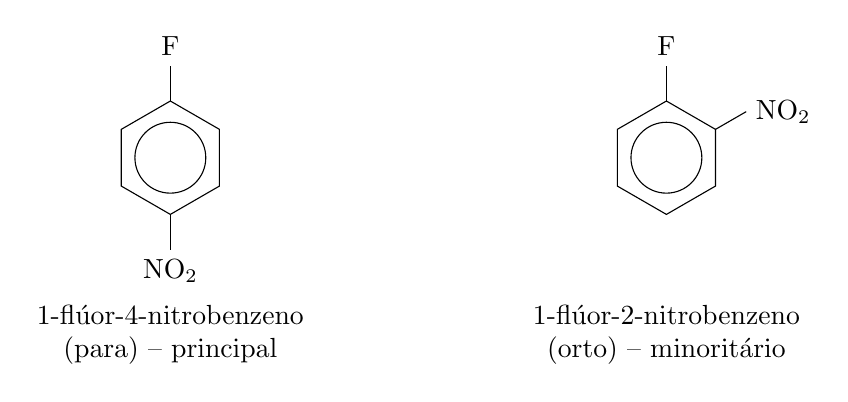
\begin{tikzpicture}[scale=0.9]
  \draw (90:0.8)--(150:0.8)--(210:0.8)--(270:0.8)--(330:0.8)--(30:0.8)--cycle;
  \draw (0,0) circle (0.5);
  \draw (90:0.8)--(90:1.3); \node[above] at (90:1.3) {F};
  \draw (270:0.8)--(270:1.3); \node[below] at (270:1.3) {NO$_2$};
  \node[align=center] at (0,-2.5) {1-flúor-4-nitrobenzeno\\(para) -- principal};
  \begin{scope}[xshift=7cm]
  \draw (90:0.8)--(150:0.8)--(210:0.8)--(270:0.8)--(330:0.8)--(30:0.8)--cycle;
  \draw (0,0) circle (0.5);
  \draw (90:0.8)--(90:1.3); \node[above] at (90:1.3) {F};
  \draw (30:0.8)--(30:1.3); \node[right] at (30:1.3) {NO$_2$};
  \node[align=center] at (0,-2.5) {1-flúor-2-nitrobenzeno\\(orto) -- minoritário};
  \end{scope}
\end{tikzpicture}
\end{center}

\medskip
\textbf{d)} (i) $\text{H}_2\text{O}$; (ii) $\text{H}_2\text{S}$; (iii) $\text{CH}_4\text{O}=\text{CH}_3\text{OH}$ (metanol, o único arranjo possível).
\begin{itemize}
\item $\text{H}_2\text{S}$ ($M=34{,}08\ \text{g/mol}$): o S é pouco eletronegativo, então não há ligações de
hidrogênio significativas, apenas dipolo--dipolo e dispersão de London $\Rightarrow$ menor ponto de
ebulição (é gás em condições ambiente, $\approx -60\ ^\circ\text{C}$).
\item $\text{CH}_3\text{OH}$ ($M=32{,}04\ \text{g/mol}$): faz ligações de hidrogênio, mas tem só
um H ligado a O $\Rightarrow$ rede de ligações de H menos extensa ($\approx 65\ ^\circ\text{C}$).
\item $\text{H}_2\text{O}$ ($M=18{,}02\ \text{g/mol}$): tem dois H ligados a O e dois pares isolados e
pode formar até 4 ligações de hidrogênio por molécula (rede tridimensional) $\Rightarrow$ maior
ponto de ebulição ($100\ ^\circ\text{C}$), mesmo tendo a menor massa molar.
\end{itemize}
Ordem crescente: $\text{H}_2\text{S}<\text{CH}_3\text{OH}<\text{H}_2\text{O}$, isto é, (ii) $<$ (iii) $<$ (i).

\medskip
ANSWER: A = H, Z = B, X = C, G = N, R = O, Y = F, Q = S. a) 3 arranjos (S--C--N, C--N--S, C--S--N); o tiocianato $[\text{SCN}]^-$ é o mais estável; b) trigonal plana: $\text{BF}_3$; pirâmide trigonal: $\text{NH}_3$; c) nitração do fluorobenzeno: 1-flúor-4-nitrobenzeno (para, principal) e 1-flúor-2-nitrobenzeno (orto); d) $\text{H}_2\text{S}<\text{CH}_3\text{OH}<\text{H}_2\text{O}$, ou seja, (ii) $<$ (iii) $<$ (i).%
\newpage%
\section*{Questão 6}

\section*{Solução}

\textbf{Relações usadas.} A $25\,^{\circ}\mathrm{C}$, para um par conjugado $\mathrm{HA}/\mathrm{A^-}$ em água vale $K_a(\mathrm{HA})\,K_b(\mathrm{A^-})=K_w$. Logo
\[
pK_a(\mathrm{HA})+pK_b(\mathrm{A^-})=pK_w=14{,}00 .
\]
Para uma reação ácido-base genérica $\mathrm{HA}+\mathrm{B}\rightleftharpoons \mathrm{A^-}+\mathrm{HB^+}$, multiplicamos e dividimos por $[\mathrm{H_3O^+}]$:
\[
K=\frac{[\mathrm{A^-}][\mathrm{HB^+}]}{[\mathrm{HA}][\mathrm{B}]}
=\frac{[\mathrm{A^-}][\mathrm{H_3O^+}]}{[\mathrm{HA}]}\cdot\frac{[\mathrm{HB^+}]}{[\mathrm{B}][\mathrm{H_3O^+}]}
=\frac{K_a(\mathrm{HA})}{K_a(\mathrm{HB^+})}
\;\Longrightarrow\;
\log K = pK_a(\text{ácido produto})-pK_a(\text{ácido reagente}).
\]
Portanto o equilíbrio favorece os produtos ($K>1$) quando o ácido formado é \emph{mais fraco} (tem $pK_a$ maior) que o ácido de partida. Uma forma equivalente é $K=K_a(\mathrm{HA})\,K_b(\mathrm{B})/K_w$, que usaremos como conferência.

\textbf{Valores das demais espécies} (a amônia é anfótera: como base, seu ácido conjugado é $\mathrm{NH_4^+}$; como ácido, sua base conjugada é $\mathrm{NH_2^-}$):

\begin{center}
\begin{tabular}{c|c||c|c}
Ácido & $pK_a$ & Base conjugada & $pK_b$\\ \hline
$\mathrm{CH_3CCH}$ & $25{,}00$ (dado) & $\mathrm{CH_3CC^-}$ & $14{,}00-25{,}00=-11{,}00$\\
$\mathrm{H_3O^+}$ & $14{,}00-15{,}70=-1{,}70$ & $\mathrm{H_2O}$ & $15{,}70$ (dado)\\
$\mathrm{NH_4^+}$ & $14{,}00-4{,}75=9{,}25$ & $\mathrm{NH_3}$ & $4{,}75$ (dado)\\
$\mathrm{NH_3}$ & $14{,}00-(-22{,}00)=36{,}00$ & $\mathrm{NH_2^-}$ & $-22{,}00$ (dado)
\end{tabular}
\end{center}

\textbf{a) Reação 1.} O ácido reagente é o propino ($pK_a=25{,}00$) e o ácido produto é o $\mathrm{H_3O^+}$ ($pK_a=-1{,}70$):
\[
\log K_1=-1{,}70-25{,}00=-26{,}70\;\Rightarrow\;K_1=10^{-26{,}70}\approx 2{,}0\times10^{-27}\ll 1 .
\]
Conferência: $K_aK_b/K_w=10^{-25{,}00}\cdot10^{-15{,}70}/10^{-14{,}00}=10^{-26{,}70}$. O $\mathrm{H_3O^+}$ é um ácido muito mais forte que o propino, e o $\mathrm{CH_3CC^-}$ ($pK_b=-11{,}00$) é uma base muito mais forte que a água ($pK_b=15{,}70$). Logo a reação \textbf{não favorece} os produtos: o propino praticamente não se ioniza em água.

\emph{Observação:} se a atividade da água for tomada como 1, a Reação 1 é a própria definição de $K_a$ do propino ($K_1=10^{-25}$). O fator $10^{-1{,}70}\approx 1/55{,}5$ de diferença vem da convenção, embutida no dado $pK_b(\mathrm{H_2O})=15{,}70$, de incluir $[\mathrm{H_2O}]=55{,}5\ \mathrm{mol\,L^{-1}}$. Em qualquer convenção, $K_1\ll1$.

\textbf{b) Reação 2.} O ácido reagente é o propino ($25{,}00$) e o ácido produto é o $\mathrm{NH_4^+}$ ($9{,}25$):
\[
\log K_2=9{,}25-25{,}00=-15{,}75\;\Rightarrow\;K_2=10^{-15{,}75}\approx 1{,}8\times10^{-16}\ll 1 .
\]
Conferência: $10^{-25{,}00}\cdot10^{-4{,}75}/10^{-14{,}00}=10^{-15{,}75}$. Como $pK_b(\mathrm{NH_3})=4{,}75$ é muito maior que $pK_b(\mathrm{CH_3CC^-})=-11{,}00$, a amônia é uma base fraca demais para desprotonar o propino. A reação \textbf{não favorece} os produtos.

\textbf{c) Reação 3.} O $\mathrm{Na^+}$ é íon espectador, e a equação iônica é $\mathrm{CH_3CCH}+\mathrm{NH_2^-}\rightleftharpoons \mathrm{CH_3CC^-}+\mathrm{NH_3}$. O ácido reagente é o propino ($25{,}00$) e o ácido produto é o $\mathrm{NH_3}$ ($36{,}00$):
\[
\log K_3=36{,}00-25{,}00=11{,}00\;\Rightarrow\;K_3=10^{11}\gg 1 .
\]
Conferência: $10^{-25{,}00}\cdot10^{22{,}00}/10^{-14{,}00}=10^{11{,}00}$. O amideto ($pK_b=-22{,}00$) é base mais forte que o propineto ($pK_b=-11{,}00$), e a amônia é ácido mais fraco que o propino. A reação \textbf{favorece} os produtos. Esse é o método usual de preparo de acetiletos (alquinetos) de sódio a partir de alquinos terminais. A reação é feita em $\mathrm{NH_3}$ líquida e não em água, porque a água, mais ácida, protonaria tanto o $\mathrm{NH_2^-}$ quanto o $\mathrm{CH_3CC^-}$.

ANSWER: $pK_b(\mathrm{CH_3CC^-})=-11{,}00$; $pK_a(\mathrm{H_3O^+})=-1{,}70$; $pK_a(\mathrm{NH_4^+})=9{,}25$; $pK_a(\mathrm{NH_3})=36{,}00$. (a) $K_1=10^{-26{,}70}\approx2{,}0\times10^{-27}$: não favorece os produtos. (b) $K_2=10^{-15{,}75}\approx1{,}8\times10^{-16}$: não favorece os produtos. (c) $K_3=10^{11}$: favorece os produtos.%
\newpage%
\section*{Questão 7}

\section*{Solução}

\textbf{Hipóteses.} Cada fóton absorvido gera um elétron (eficiência quântica de 100\%). A energia de um fóton é $E=\dfrac{hc}{\lambda}$ (equação de Planck--Einstein). Massa molar: $M(\text{H}_2)=2\cdot 1{,}01=2{,}02\ \text{g/mol}$.

\medskip
\textbf{a) Semirreações.} No cátodo ocorre redução e no ânodo, oxidação. Em meio ácido:
\begin{align*}
\text{Cátodo (redução):}&\quad 4\,\text{H}^+(\text{aq}) + 4\,e^- \rightarrow 2\,\text{H}_2(\text{g})\\
\text{Ânodo (oxidação):}&\quad 2\,\text{H}_2\text{O}(\ell) \rightarrow \text{O}_2(\text{g}) + 4\,\text{H}^+(\text{aq}) + 4\,e^-\\
\text{Global:}&\quad 2\,\text{H}_2\text{O}(\ell) \rightarrow 2\,\text{H}_2(\text{g}) + \text{O}_2(\text{g})
\end{align*}
(Em meio básico: cátodo $4\,\text{H}_2\text{O} + 4\,e^- \rightarrow 2\,\text{H}_2 + 4\,\text{OH}^-$; ânodo $4\,\text{OH}^- \rightarrow \text{O}_2 + 2\,\text{H}_2\text{O} + 4\,e^-$, com a mesma equação global.) Logo, cada mol de H$_2$ exige 2 mol de elétrons, ou seja, 2 mol de fótons.

\medskip
\textbf{b) Energia luminosa por mol de H$_2$.} Energia de um fóton de 450 nm:
\[
E_f=\frac{hc}{\lambda}=\frac{6{,}63\times10^{-34}\cdot 3{,}0\times10^{8}}{450\times10^{-9}}=4{,}42\times10^{-19}\ \text{J}\quad(\approx 2{,}76\ \text{eV}).
\]
Por mol de fótons: $N_A E_f = 6{,}02\times10^{23}\cdot 4{,}42\times10^{-19}=2{,}66\times10^{5}\ \text{J}$. Como são necessários 2 mol de fótons por mol de H$_2$:
\[
E_{\text{H}_2}=2\cdot 2{,}66\times10^{5}\ \text{J}=5{,}32\times10^{5}\ \text{J}=532\ \text{kJ por mol de H}_2 .
\]
Verificação: o valor supera $\Delta H^\circ/2=286\ \text{kJ}$ por mol de H$_2$, portanto a energia dos fótons de 450 nm é suficiente para a decomposição.

\medskip
\textbf{c) Máximo de H$_2$ em 1 h.} Energia luminosa recebida (potência $\times$ área $\times$ tempo):
\[
E_{\text{luz}}=10\cdot 0{,}2\cdot 3600=7{,}2\times10^{3}\ \text{J}.
\]
Número de fótons: $N=\dfrac{7{,}2\times10^{3}}{4{,}42\times10^{-19}}=1{,}63\times10^{22}$, ou seja, $n_{e^-}=\dfrac{1{,}63\times10^{22}}{6{,}02\times10^{23}}=2{,}71\times10^{-2}\ \text{mol}$ de elétrons. Então
\[
n_{\text{H}_2}=\frac{n_{e^-}}{2}=1{,}35\times10^{-2}\ \text{mol}
\]
(equivalentemente, $7200\ \text{J}/(5{,}32\times10^{5}\ \text{J/mol})=1{,}35\times10^{-2}\ \text{mol}$).

\medskip
\textbf{d) Energia para encher o tanque.} Quantidade de H$_2$ (desprezando efeitos de pressão):
\[
n=\frac{5650\ \text{g}}{2{,}02\ \text{g/mol}}=2{,}80\times10^{3}\ \text{mol}.
\]
O semicondutor só absorve fótons com $\lambda\le 450$ nm. Como $E_f$ diminui com $\lambda$, a energia mínima corresponde a fótons de exatamente 450 nm, isto é, 532 kJ por mol de H$_2$ (item b):
\[
E_{\min}=2{,}80\times10^{3}\cdot 5{,}32\times10^{5}\ \text{J}\approx 1{,}49\times10^{9}\ \text{J}=1{,}49\ \text{GJ}.
\]

\medskip
\textbf{e) Comprimento de onda hipotético.} Na combustão $2\,\text{H}_2 + \text{O}_2 \rightarrow 2\,\text{H}_2\text{O}(\ell)$, $\Delta H^\circ=-572$ kJ, ou seja, são liberados 286 kJ por mol de H$_2$. Para os $2{,}80\times10^{3}$ mol:
\[
E_{\text{comb}}=2{,}80\times10^{3}\cdot 286\ \text{kJ}\approx 8{,}0\times10^{5}\ \text{kJ}.
\]
Igualando essa energia à dos fótons ($2n$ mol de fótons, proporção 1:1 com os elétrons, sem perdas), a energia por mol de fótons é
\[
\frac{8{,}0\times10^{5}\ \text{kJ}}{2\cdot 2{,}80\times10^{3}\ \text{mol}}=\frac{286}{2}=143\ \text{kJ/mol}.
\]
Logo,
\[
\lambda_{\max}=\frac{N_A hc}{143\times10^{3}}=\frac{6{,}02\times10^{23}\cdot 6{,}63\times10^{-34}\cdot 3{,}0\times10^{8}}{1{,}43\times10^{5}}=\frac{0{,}1197}{1{,}43\times10^{5}}\ \text{m}\approx 8{,}37\times10^{-7}\ \text{m}\approx 837\ \text{nm}.
\]
Coerência: $837\ \text{nm}>450\ \text{nm}$ (infravermelho próximo, cerca de $1{,}48$ eV por fóton). Fótons de menor energia bastariam no caso ideal, e a eficiência do semicondutor real seria $286/532\approx 54\%$.

\medskip
ANSWER: a) Cátodo: $4\text{H}^+ + 4e^- \rightarrow 2\text{H}_2$; ânodo: $2\text{H}_2\text{O} \rightarrow \text{O}_2 + 4\text{H}^+ + 4e^-$. b) $\approx 5{,}32\times10^{5}$ J (532 kJ) por mol de H$_2$. c) $\approx 1{,}35\times10^{-2}$ mol de H$_2$. d) $\approx 1{,}49\times10^{9}$ J. e) $\lambda_{\max}\approx 837$ nm.%
\newpage%
\section*{Questão 8}

\section*{Solução}

\textbf{Dados auxiliares.} $M(\text{CH}_4)=12{,}01+4\cdot 1{,}01=16{,}05\ \text{g/mol}$; $M(\text{O}_2)=32{,}00\ \text{g/mol}$.

Pelo requisito I, a água sai como gás. Pela lei de Hess (vaporização somada à formação do líquido):
\[
\Delta H_f(\text{H}_2\text{O(g)})=-286+45=-241\ \text{kJ/mol}.
\]

\textbf{a)} Combustão completa com todos os produtos gasosos:
\[
\text{CH}_4(\text{g})+2\,\text{O}_2(\text{g})\longrightarrow \text{CO}_2(\text{g})+2\,\text{H}_2\text{O}(\text{g})
\]
\[
\Delta H_c=\left[-393+2(-241)\right]-\left[-75+2\cdot 0\right]=-875+75=-800\ \text{kJ/mol de CH}_4 .
\]
A reação é exotérmica e libera $800$ kJ por mol de CH$_4$. Para gerar $12\ \text{MJ}$, a variação de entalpia do processo é $\Delta H=-12\ \text{MJ}$, o que corresponde à queima de $n=12000/800=15$ mol de CH$_4$.

\textbf{b)} Os dados termodinâmicos não dependem de $T$ e $p$, e o calor liberado é proporcional à quantidade queimada:
\[
n_{\text{CH}_4}=\frac{12000\ \text{kJ}}{800\ \text{kJ/mol}}=15\ \text{mol}\ \Rightarrow\ m_{\text{CH}_4}=15\cdot 16{,}05=240{,}75\ \text{g}\approx 241\ \text{g}.
\]
\[
n_{\text{O}_2}=2\cdot 15=30\ \text{mol}\ \Rightarrow\ m_{\text{O}_2}=30\cdot 32{,}00=960\ \text{g}.
\]

\textbf{c)} A turbobomba pressuriza o combustível que será queimado na câmara principal, isto é, os $240{,}75$ g do item b. A energia útil necessária é:
\[
E_{\text{útil}}=40\ \tfrac{\text{J}}{\text{g}}\cdot 240{,}75\ \text{g}=9630\ \text{J}.
\]
Como a eficiência é de $30\%$, o calor gerado na pré-câmara deve ser:
\[
Q_{\text{pré}}=\frac{9630}{0{,}30}=32100\ \text{J}=32{,}1\ \text{kJ}.
\]
A pré-câmara queima CH$_4$ pela mesma reação do item a ($-800$ kJ/mol):
\[
n=\frac{32{,}1}{800}=4{,}0125\cdot 10^{-2}\ \text{mol}\ \Rightarrow\ m=4{,}0125\cdot 10^{-2}\cdot 16{,}05\approx 0{,}644\ \text{g}.
\]
Isso equivale a cerca de $0{,}27\%$ do combustível, o que confirma a ``pequena porcentagem'' do enunciado. Essa queima consome mais $2\cdot 0{,}0401\ \text{mol}\approx 2{,}57$ g de O$_2$. Isso explica por que a mistura que sai da pré-câmara é rica em O$_2$: a maior parte do oxidante passa sem reagir para a câmara principal.

Se, em outra leitura, os $240{,}75$ g incluíssem o combustível da pré-câmara, teríamos $0{,}3\cdot\tfrac{800000}{16{,}05}\,m=40\,(240{,}75-m)$, o que dá $m\approx 0{,}642$ g. O resultado é praticamente o mesmo.

\textbf{d)} Calor que a tubeira absorve:
\[
Q_{\text{tub}}=0{,}25\%\cdot 12\ \text{MJ}=0{,}0025\cdot 1{,}2\cdot 10^{7}\ \text{J}=3{,}0\cdot 10^{4}\ \text{J}.
\]
Esse calor é retirado pelo CH$_4$ como calor sensível, já que o enunciado manda desprezar a energia da mudança de fase. A massa será mínima quando o metano for aquecido até o limite de $188$ K, partindo de $98$ K:
\[
Q=m\,c\,\Delta T \Rightarrow m_{\min}=\frac{3{,}0\cdot 10^{4}}{\tfrac{5}{3}\cdot(188-98)}=\frac{3{,}0\cdot 10^{4}}{150}=200\ \text{g}.
\]
Verificação: $200\ \text{g}<240{,}75\ \text{g}$. Portanto, o próprio combustível bombeado para a câmara basta para refrigerar a tubeira, o que é coerente com o esquema do motor.

ANSWER: a) $\text{CH}_4+2\,\text{O}_2\to\text{CO}_2+2\,\text{H}_2\text{O(g)}$, $\Delta H_c=-800\ \text{kJ/mol}$ ($\Delta H=-12$ MJ para 15 mol de CH$_4$); b) $m_{\text{CH}_4}\approx 240{,}75\ \text{g}$ e $m_{\text{O}_2}=960\ \text{g}$; c) $\approx 0{,}644\ \text{g}$ de CH$_4$(g); d) $200\ \text{g}$ de CH$_4$(l).%
\newpage%
\section*{Questão 9}

\section*{Solução}

\textbf{Ideia central.} O experimento é a clássica demonstração da \emph{migração iônica}. A mistura é marrom porque reúne o azul do $\text{Cu}^{2+}$ hidratado e o alaranjado do $\text{Cr}_2\text{O}_7^{2-}$. Por ser mais densa, ela fica no fundo do U. O $\text{H}_2\text{SO}_4$ diluído (incolor) foi colocado com cuidado por cima e serve de eletrólito condutor em contato com as placas. Sob o campo elétrico da fonte, os cátions migram para o catodo (eletrodo negativo) e os ânions para o anodo (eletrodo positivo).

\medskip
\textbf{a) Espécies iônicas presentes.}
\begin{itemize}
\item Cátions: $\text{Cu}^{2+}$ (na forma $[\text{Cu}(\text{H}_2\text{O})_6]^{2+}$, azul), $\text{K}^{+}$ e $\text{H}^{+}$ (ou $\text{H}_3\text{O}^{+}$), este último vindo do ácido sulfúrico.
\item Ânions: $\text{SO}_4^{2-}$ (do $\text{CuSO}_4$ e do ácido), $\text{HSO}_4^{-}$ (2ª ionização do $\text{H}_2\text{SO}_4$ é parcial) e $\text{Cr}_2\text{O}_7^{2-}$ (alaranjado).
\item Em quantidades muito pequenas: $\text{OH}^{-}$ (autoionização da água) e $\text{HCrO}_4^{-}$ ou $\text{CrO}_4^{2-}$, vindos do equilíbrio
$\text{Cr}_2\text{O}_7^{2-} + \text{H}_2\text{O} \rightleftharpoons 2\,\text{HCrO}_4^{-} \rightleftharpoons 2\,\text{CrO}_4^{2-} + 2\,\text{H}^{+}$. Em meio ácido, esse equilíbrio fica deslocado para o dicromato.
\end{itemize}

\textbf{b) Origem das camadas azul e alaranjada.}
Os íons coloridos têm cargas de sinais opostos e, por isso, migram em sentidos opostos. O $\text{Cu}^{2+}$ (azul) sobe pelo braço do catodo, e o $\text{Cr}_2\text{O}_7^{2-}$ (alaranjado) sobe pelo braço do anodo.

No braço do catodo, a frente que avança para dentro da camada incolor de $\text{H}_2\text{SO}_4$ só contém $\text{Cu}^{2+}$, porque o $\text{Cr}_2\text{O}_7^{2-}$ desse braço é afastado para baixo. Surge então a faixa azul. No outro braço ocorre o inverso: só o $\text{Cr}_2\text{O}_7^{2-}$ avança para cima, formando a faixa alaranjada. No fundo do U, as duas espécies continuam juntas e a cor segue marrom.

Os demais íons ($\text{K}^{+}$, $\text{H}^{+}$, $\text{SO}_4^{2-}$, $\text{HSO}_4^{-}$) são incolores. A migração é lenta, por isso a região das placas ainda está incolor.

\medskip
\textbf{c) Anodo, catodo e semirreações.}
A faixa azul ($\text{Cu}^{2+}$, cátion) aparece no braço de $\text{Pt}_1$. Logo, $\text{Pt}_1$ atrai cátions: é o \textbf{catodo}, onde ocorre redução. A faixa alaranjada ($\text{Cr}_2\text{O}_7^{2-}$, ânion) aparece no braço de $\text{Pt}_2$. Logo, $\text{Pt}_2$ é o \textbf{anodo}, onde ocorre oxidação.

As placas estão em contato com o $\text{H}_2\text{SO}_4$ diluído, que contém $\text{H}^{+}$, $\text{HSO}_4^{-}$, $\text{SO}_4^{2-}$ e $\text{H}_2\text{O}$.

\emph{Catodo ($\text{Pt}_1$).} O $\text{H}^{+}$ ($E^\circ = 0{,}00\ \text{V}$) se reduz muito mais facilmente que o $\text{K}^{+}$ ($E^\circ \approx -2{,}9\ \text{V}$):
\[
2\,\text{H}^{+}(\text{aq}) + 2\,e^{-} \rightarrow \text{H}_2(\text{g}).
\]
Se o $\text{Cu}^{2+}$ chegasse até a placa, sua redução, $\text{Cu}^{2+} + 2e^{-} \rightarrow \text{Cu}(\text{s})$ com $E^\circ = +0{,}34\ \text{V}$, passaria a ser a preferencial. Na Figura (B), porém, a região da placa ainda está incolor.

\emph{Anodo ($\text{Pt}_2$).} A Pt é inerte. A água ($E^\circ_{\text{O}_2/\text{H}_2\text{O}} = 1{,}23\ \text{V}$) se oxida antes do sulfato, que só formaria $\text{S}_2\text{O}_8^{2-}$ com $E^\circ = 2{,}01\ \text{V}$:
\[
2\,\text{H}_2\text{O}(\ell) \rightarrow \text{O}_2(\text{g}) + 4\,\text{H}^{+}(\text{aq}) + 4\,e^{-}.
\]
O dicromato que se aproxima do anodo não pode ser oxidado, pois o Cr já está em seu número de oxidação máximo, $+6$.

Reação global: $2\,\text{H}_2\text{O} \rightarrow 2\,\text{H}_2 + \text{O}_2$. É a eletrólise da água, e o $\text{H}_2\text{SO}_4$ atua só como eletrólito.

\medskip
\textbf{d) Polaridade da fonte e sentido da corrente.}
O catodo é ligado ao polo negativo, que lhe fornece elétrons. Assim, \textbf{$\text{P}_1$ é negativo} e \textbf{$\text{P}_2$ é positivo}.
\begin{itemize}
\item Elétrons no fio: saem de $\text{P}_1$ e vão a $\text{Pt}_1$, onde são consumidos na redução. Os liberados na oxidação em $\text{Pt}_2$ seguem para $\text{P}_2$.
\item Corrente convencional, de sentido oposto ao dos elétrons: $\text{P}_2\ (+) \rightarrow \text{Pt}_2 \rightarrow$ solução $\rightarrow \text{Pt}_1 \rightarrow \text{P}_1\ (-)$, fechando o circuito dentro da fonte de $\text{P}_1$ para $\text{P}_2$.
\item Na solução, a corrente é conduzida pelos íons: cátions de $\text{Pt}_2$ para $\text{Pt}_1$ e ânions de $\text{Pt}_1$ para $\text{Pt}_2$. Isso é coerente com as faixas observadas.
\end{itemize}

\medskip
ANSWER: a) $\text{Cu}^{2+}$, $\text{K}^{+}$, $\text{H}^{+}$ ($\text{H}_3\text{O}^{+}$), $\text{SO}_4^{2-}$, $\text{HSO}_4^{-}$ e $\text{Cr}_2\text{O}_7^{2-}$, além de traços de $\text{OH}^{-}$, $\text{HCrO}_4^{-}$ e $\text{CrO}_4^{2-}$. b) Pela migração iônica, o $\text{Cu}^{2+}$ (azul) vai para o catodo e o $\text{Cr}_2\text{O}_7^{2-}$ (alaranjado) vai para o anodo, separando as cores que juntas davam o marrom. c) $\text{Pt}_1$ é o catodo: $2\text{H}^{+} + 2e^{-} \rightarrow \text{H}_2$; o $\text{Cu}^{2+} + 2e^{-} \rightarrow \text{Cu}$ passaria a ser preferencial se o cobre chegasse à placa. $\text{Pt}_2$ é o anodo: $2\text{H}_2\text{O} \rightarrow \text{O}_2 + 4\text{H}^{+} + 4e^{-}$. d) $\text{P}_1$ é negativo e $\text{P}_2$ é positivo; a corrente convencional vai de $\text{P}_2 \rightarrow \text{Pt}_2 \rightarrow$ solução $\rightarrow \text{Pt}_1 \rightarrow \text{P}_1$, e os elétrons vão de $\text{P}_1$ para $\text{Pt}_1$ e de $\text{Pt}_2$ para $\text{P}_2$.%
\newpage%
\section*{Questão 10}

\section*{Solução}

\textbf{Leis usadas.} Em qualquer decaimento nuclear o número de massa (núcleons) e a carga se conservam:
\begin{itemize}
\item emissão $\alpha$ (${}^{4}_{2}\alpha$): o núcleo perde 4 unidades de massa e 2 prótons;
\item emissão $\beta^-$ (${}^{\ 0}_{-1}\beta$): um nêutron vira próton, $n \rightarrow p + e^- + \bar{\nu}$, então a massa não muda e $Z$ aumenta em 1.
\end{itemize}
Também usamos $N = A - Z$ (número de nêutrons). Definições: \emph{isóbaros} têm o mesmo número de massa $A$; \emph{isótonos} têm o mesmo número de nêutrons $N$.

\medskip
\textbf{1) Elemento G (consideração iii).} G vem de um decaimento $\beta^-$ de ${}^{232}_{\ 89}\text{Q}$:
\[
{}^{232}_{\ 89}\text{Q} \rightarrow {}^{\ \ 0}_{-1}\beta + {}^{232}_{\ 90}\text{G}
\qquad (232 = 0 + 232;\quad 89 = -1 + 90).
\]
Número de nêutrons de G: $N_G = 232 - 90 = 142$.

\medskip
\textbf{2) Elemento E (considerações ii e iv).} E é isótono de G, logo $N_E = 142$. Como E tem $Z_E = 84$ prótons:
\[
A_E = Z_E + N_E = 84 + 142 = 226 \quad\Rightarrow\quad {}^{226}_{\ 84}\text{E}.
\]

\medskip
\textbf{a) Massa X (consideração i).} A é isóbaro de E, então tem o mesmo número de massa:
\[
X = A_E = 226 .
\]

\medskip
\textbf{c) Número de partículas $\alpha$.} J (${}^{238}_{\ 92}\text{J}$) só emite partículas $\alpha$. Com $n$ emissões, a conservação do número de massa dá
\[
238 = X + 4n = 226 + 4n \;\Rightarrow\; 4n = 12 \;\Rightarrow\; n = 3 .
\]

\medskip
\textbf{b) Número atômico Z.} A conservação da carga nas 3 emissões $\alpha$ dá
\[
92 = Z + 2n = Z + 2 \cdot 3 \;\Rightarrow\; Z = 92 - 6 = 86 .
\]
O processo completo é
\[
{}^{238}_{\ 92}\text{J} \rightarrow 3\,{}^{4}_{2}\alpha + {}^{226}_{\ 86}\text{A}.
\]

\medskip
\textbf{Verificação.} Massa: $3\cdot 4 + 226 = 238$. Carga: $3\cdot 2 + 86 = 92$. A tem $226$ núcleons, como E, e por isso os dois são isóbaros. Eles diferem em $Z$ ($86 \neq 84$), portanto são elementos diferentes, como pede a definição. $Z = 86$ é o radônio. Assim, $J = {}^{238}\text{U}$, $Q = {}^{232}\text{Ac}$, $G = {}^{232}\text{Th}$ e $E = {}^{226}\text{Po}$, todos com números de prótons coerentes.

\medskip
ANSWER: a) $X = 226$; \ b) $Z = 86$; \ c) 3 partículas $\alpha$.%
\newpage%
\section*{Apêndice: parecer do avaliador}%
\subsection*{Questão 1: nota 9,5 (aprovada, rodada 1 de 1)}%
\textbf{Resposta da resolução às cegas do avaliador:} a) {[}HA{]} na Solução 2 = 0,4 mol/L\newline%
b) {[}HA{]} na Solução 1 = 2 mol/L\newline%
c) {[}base{]} na Solução 3 = 8$\times$10$^{-}$$^{4}$/0,038 = 2/95 $\approx$ 0,021 mol/L ($\approx$ 2,1$\times$10$^{-}$$^2$ mol/L)\newline%
\newline%
Base de cálculo: no ponto de equivalência só há A$^{-}$ em 40 mL. Kb = Kw/Ka = 10$^{-}$$^2$. pH = 12 dá {[}OH$^{-}${]} = {[}HA{]} = 10$^{-}$$^2$. Pela expressão completa, 10$^{-}$$^2$ = (10$^{-}$$^2$)$^2$/(C - 10$^{-}$$^2$), logo C = 2$\times$10$^{-}$$^2$ mol/L, porque o ânion está 50 \% hidrolisado. Então n = 8$\times$10$^{-}$$^{4}$ mol. Se o candidato usar a aproximação C - x $\approx$ C, encontra 0,2; 1,0 e 1,05$\times$10$^{-}$$^2$ mol/L, todos com erro de um fator 2.\par %
Comparei as respostas item por item com a minha referência e todas coincidem: a) 0,4 mol/L; b) 2 mol/L; c) 2/95 $\approx$ 2,1$\times$10$^{-}$$^2$ mol/L. Conferi a transcrição com a página 3 do PDF e ela está fiel. Também refiz o balanço de cargas exato em python: C(sal) = 0,0200 mol/L, n = 8,0$\times$10$^{-}$$^{4}$ mol, C$_{2}$ = 0,400, C$_{1}$ = 2,00 e C$_{3}$ = 0,02105 mol/L.\newline%
\newline%
O candidato tratou todas as armadilhas:\newline%
{-} Declarou Kw = 10$^{-}$$^{1}$$^{4}$ e calculou Kb = 10$^{-}$$^2$.\newline%
{-} Recusou explicitamente a aproximação C - x $\approx$ C e usou o balanço de massa C = {[}A$^{-}${]} + {[}HA{]}. Com isso obteve 2$\times$10$^{-}$$^2$ mol/L e não o valor errado 10$^{-}$$^2$, e ainda comentou que o ânion está 50 \% hidrolisado.\newline%
{-} Atribuiu o pH à hidrólise e não a um excesso de base.\newline%
{-} Usou o volume total de 40 mL.\newline%
{-} Aplicou a diluição com fator 5 no sentido correto (C$_{1}$ = 5$\cdot$C$_{2}$).\newline%
{-} No item c dividiu por 38 mL, sem confundir com a concentração do sal.\newline%
{-} Deu todas as respostas com unidade e com as expressões numéricas resolvidas até o fim.\newline%
\newline%
Ficam só ressalvas menores de rigor e de redação: a verificação final é quase circular, a expressão 'Kb grande' é imprecisa e as hipóteses (volumes aditivos, idealidade, 'Solução I' = Solução 1) não foram declaradas. É uma resolução clara e correta, que poderia ser publicada como gabarito comentado.%
\begin{itemize}%
\item%
{[}minor{]} A 'verificação' pelo balanço de cargas é quase circular. Ela usa {[}A$^{-}${]} e {[}OH$^{-}${]} tirados das mesmas hipóteses ({[}HA{]} = {[}OH$^{-}${]}) e só confirma a coerência interna. Não é uma verificação independente. O ideal seria partir do balanço exato: C + {[}H?{]} = {[}A$^{-}${]} + {[}OH$^{-}${]} com {[}A$^{-}${]} = C$\cdot$Ka/(Ka + {[}H?{]}). Isso dá C = 2(10$^{-}$$^2$ - 10$^{-}$$^{1}$$^2$) $\approx$ 2$\times$10$^{-}$$^2$ mol/L e mostra que a aproximação {[}HA{]} = {[}OH$^{-}${]} é exata até 10$^{-}$$^{1}$$^2$.%
\item%
{[}minor{]} A frase 'Como K\_b é grande' é imprecisa: 10$^{-}$$^2$ não é grande em termos absolutos. O critério certo é comparar a fração hidrolisada x/C (ou Kb com C): com {[}OH$^{-}${]} = 10$^{-}$$^2$ e C da mesma ordem, C - x $\approx$ C não vale. A conclusão está certa e a conta exata foi feita, então o efeito no resultado é nulo.%
\item%
{[}minor{]} Hipóteses usadas sem declarar: volumes aditivos (V = 2 + 38 = 40 mL), comportamento ideal (atividade igual a concentração, o que merece ressalva com C$_{1}$ = 2 mol/L) e que a 'Solução I' do enunciado é a Solução 1. Bastaria uma linha de hipóteses.%
\end{itemize}%
\subsection*{Questão 2: nota 9,5 (aprovada, rodada 1 de 1)}%
\textbf{Resposta da resolução às cegas do avaliador:} a) n(H$_{2}$O$_{2}$) = 0,050 mol, então n(O$_{2}$) = 0,025 mol. V = nRT/P = 0,025 $\times$ 0,0821 $\times$ 298/1 $\approx$ 0,61 L ($\approx$ 612 mL) de O$_{2}$ a 25 $^\circ$C e 1 atm.\newline%
b) A unidade min$^{-}$$^{1}$ indica 1ª ordem: {[}H$_{2}$O$_{2}${]} = 0,5$\cdot$e\^{}(-0,0693$\times$5) = 0,5 $\times$ 0,707 $\approx$ 0,35 mol$\cdot$L$^{-}$$^{1}$ (0,354 mol$\cdot$L$^{-}$$^{1}$). Pela meia{-}vida: t$_{1}$/$_{2}$ = 10 min, logo 0,5/$\surd$2.\par %
Conferi o enunciado na página 4 do PDF: ele é igual à transcrição.\newline%
\newline%
**Respostas finais, item por item.** As do candidato coincidem com as da minha referência:\newline%
{-} **a)** V(O$_{2}$) = 0,025$\cdot$0,0821$\cdot$298 $\approx$ 0,612 L. O valor exato da conta é 0,6116 L.\newline%
{-} **b)** {[}H$_{2}$O$_{2}${]} = 0,5$\cdot$e\^{}(-0,3465) = 0,5$\cdot$0,707 $\approx$ 0,354 mol$\cdot$L$^{-}$$^{1}$. O valor exato é 0,3535 mol$\cdot$L$^{-}$$^{1}$.\newline%
\newline%
Refiz as contas em python3 e não há erro numérico.\newline%
\newline%
**Armadilhas tratadas.** O candidato cobriu todas:\newline%
{-} Deduz a 1ª ordem pela unidade de k e explica isso pela análise dimensional de v = k{[}H$_{2}$O$_{2}${]}.\newline%
{-} Diz explicitamente que k se refere ao consumo de H$_{2}$O$_{2}$. Assim evita a armadilha do fator 2 que levaria a 0,25 M.\newline%
{-} Aplica a estequiometria 2:1 e obtém 0,025 mol de O$_{2}$.\newline%
{-} Usa 298 K e nRT/P em vez de 22,4 L, e ainda compara com o valor nas CNTP.\newline%
{-} Interpreta 'ao término da reação' como conversão completa e observa que o catalisador não muda a quantidade de produto.\newline%
{-} Calcula kt = 0,3465 sem fator 60 e usa o dado e\^{}(-0,3465) = 0,707 fornecido pela prova.\newline%
{-} Dá a resposta em concentração.\newline%
{-} Resolve todas as expressões numéricas, como pede a instrução 8.\newline%
{-} Confere o resultado pela meia{-}vida (t$_{1}$/$_{2}$ = 10 min).\newline%
\newline%
**Falhas.** São apenas de rigor e redação:\newline%
{-} Não diz que o O$_{2}$ é seco (despreza a pressão de vapor da água).\newline%
{-} Não diz que o volume da solução fica constante.\newline%
{-} Há uma frase ambígua na conferência pela meia{-}vida.\newline%
\newline%
**Avaliação geral.** A resolução é clara, bem organizada e tem nível de gabarito comentado.%
\begin{itemize}%
\item%
{[}minor{]} Item a: o candidato considera o O$_{2}$ gás ideal e despreza a solubilidade, mas não diz que o volume é de O$_{2}$ seco, isto é, que se despreza a pressão de vapor da água a 25 $^\circ$C. Bastava uma frase dizendo que o volume pedido é o do O$_{2}$ puro (seco).%
\item%
{[}minor{]} Item b: falta dizer que o volume da solução fica constante em 100 mL. Sem isso, não se justifica tratar {[}H$_{2}$O$_{2}${]} como grandeza que só varia pela reação. Basta uma linha registrando essa hipótese.%
\item%
{[}minor{]} Na conferência pela meia{-}vida, a frase 'O resultado fica entre 0,5 e 0,25 mol L$^{-}$$^{1}$, que é o valor esperado em t = t$_{1}$/$_{2}$' é ambígua: dá a entender que o resultado (0,354) é o valor em t$_{1}$/$_{2}$, quando quem é o valor em t$_{1}$/$_{2}$ é 0,25. Além disso, a conferência por 2\^{}(-1/2) $\approx$ 0,707 só repete o dado da prova, então é coerente mas não é uma verificação independente. Deveria dizer: 'fica entre 0,5 (t = 0) e 0,25 (t = t$_{1}$/$_{2}$)'.%
\item%
{[}minor{]} O volume molar de 24,5 L/mol a 25 $^\circ$C e 1 atm, usado na conferência do item a, não vem da prova. Como serve só de checagem e coincide com nRT/P, não pesa, mas convém indicar que sai de RT/P = 0,0821$\cdot$298 $\approx$ 24,5 L/mol.%
\end{itemize}%
\subsection*{Questão 3: nota 9,5 (aprovada, rodada 1 de 1)}%
\textbf{Resposta da resolução às cegas do avaliador:} a) A precipitação começa quando o volume cai para V = $\surd$0,2 L $\approx$ 0,447 L, ou seja, depois de evaporar cerca de 552 g de água. Como a fonte evapora 1 g/s, t $\approx$ 552 s (553 s com $\surd$5 exato; $\approx$ 5,5$\cdot$10$^2$ s).\newline%
b) Com V = V$_{1}$/2 $\approx$ 0,224 L e cerca de 6,35$\cdot$10$^{-}$$^{4}$ mol de AB precipitado: {[}A?{]} = $\surd$5(1+$\surd$3)$\cdot$10$^{-}$$^3$ $\approx$ 6,1$\cdot$10$^{-}$$^3$ mol/L e {[}B$^{-}${]} = $\surd$5($\surd$3-1)$\cdot$10$^{-}$$^3$ $\approx$ 1,6$\cdot$10$^{-}$$^3$ mol/L. O produto é 1$\cdot$10$^{-}$$^{5}$ = K\_ps.\par %
Conferi o enunciado no PDF (página 5) e a transcrição está fiel. As respostas finais do candidato coincidem com as da minha referência item por item.\newline%
\newline%
(a) A precipitação começa em V* = $\surd$0,2 L $\approx$ 0,447 L. A água evaporada é $\approx$ 552,8 g e a taxa de evaporação é 1 g/s, então t $\approx$ 552 s com $\surd$5 = 2,24, ou 553 s com $\surd$5 exato.\newline%
\newline%
(b) Com V$_{2}$ = V*/2 = $\surd$5/10 L, a equação de equilíbrio é (2$\cdot$10$^{-}$$^3$ - x)(1$\cdot$10$^{-}$$^3$ - x) = 5$\cdot$10$^{-}$$^{7}$, que dá y = (3 $\pm$ $\surd$3)/2. A raiz y $\approx$ 2,37 é corretamente descartada. Ficam {[}A?{]} = $\surd$5(1+$\surd$3)$\cdot$10$^{-}$$^3$ $\approx$ 6,1$\cdot$10$^{-}$$^3$ mol/L e {[}B$^{-}${]} = $\surd$5($\surd$3-1)$\cdot$10$^{-}$$^3$ $\approx$ 1,6$\cdot$10$^{-}$$^3$ mol/L. Conferi em Python: 6,109$\cdot$10$^{-}$$^3$ e 1,637$\cdot$10$^{-}$$^3$, com produto 1,0$\cdot$10$^{-}$$^{5}$ e diferença 4,472$\cdot$10$^{-}$$^3$.\newline%
\newline%
Todas as armadilhas foram tratadas:\newline%
{-} verificou que Q$_{0}$ = 2$\cdot$10$^{-}$$^{6}$ < K\_ps;\newline%
{-} não somou calor sensível e obteve a taxa de 1 g/s;\newline%
{-} distinguiu volume restante de volume evaporado;\newline%
{-} usou quantidades em mol constantes antes da precipitação;\newline%
{-} tomou a metade de V*, e não do volume inicial;\newline%
{-} resolveu o equilíbrio em vez de tratar a reação como completa;\newline%
{-} escolheu a raiz física;\newline%
{-} não supôs concentrações fixas depois da saturação. A verificação de que n\_A - n\_B se conserva deixa isso claro.\newline%
\newline%
A apresentação é limpa, com forma exata e valores numéricos usando as aproximações fornecidas na prova. Há verificação final de K\_ps e de x < n\_B. Só restam ressalvas pequenas: o uso impróprio de 'ordem de grandeza', a frase que afirma a presença de AB(s) em V$_{2}$ sem justificativa explícita, e a falta de um comentário descartando a leitura 'metade de 1 L'. A resolução está em nível de gabarito comentado.%
\begin{itemize}%
\item%
{[}minor{]} Em (a), a frase 'a ordem de grandeza é de cerca de 9 min' usa o termo errado. 552 s $\approx$ 9,2 min é uma conversão de unidade; ordem de grandeza seria 10$^2$ s. Deveria dizer apenas 't $\approx$ 552 s $\approx$ 9,2 min'.%
\item%
{[}minor{]} Em (b), o candidato apenas afirma que 'agora a solução está saturada e em equilíbrio com AB(s)'. Faltou justificar em uma linha: depois de V*, sem precipitação o produto iônico 2$\cdot$10$^{-}$$^{6}$/V$^2$ passaria de K\_ps, então AB(s) tem de existir. Também caberia notar explicitamente que x > 0 confirma isso. A conclusão está certa, só falta o argumento.%
\item%
{[}minor{]} Para deixar clara a interpretação de 'metade', o candidato poderia comentar que tomar metade do volume inicial (0,5 L) não faria sentido, pois aí Q = 8$\cdot$10$^{-}$$^{6}$ < K\_ps e ainda não há sólido. A leitura adotada (V*/2) está correta, mas o comentário mostraria que a alternativa foi considerada e descartada.%
\end{itemize}%
\subsection*{Questão 4: nota 9,5 (aprovada, rodada 1 de 1)}%
\textbf{Resposta da resolução às cegas do avaliador:} a) Para 10 g de BGN são necessários cerca de 1,59 g de Nb$_{2}$O$_{5}$ (5,98 $\times$ 10$^{-}$$^3$ mol). A massa de oxalato amoniacal de nióbio hidratado é 1,59/0,285 $\approx$ 5,58 g ($\approx$ 5,6 g). Com n = 9 exato, dá 5,56 g, também aceitável.\newline%
b) A massa molar obtida pela termogravimetria é $\approx$ 466 g/mol. Como o sal anidro tem 303,0 g/mol, n = (466,35 - 303,00)/18,02 $\approx$ 9,06, ou seja, n = 9: NH$_{4}${[}NbO(C$_{2}$O$_{4}$)$_{2}${]}$\cdot$9H$_{2}$O.\par %
Conferi o enunciado na página 6 da prova original e ele bate com a transcrição. As respostas do candidato coincidem com a minha referência nos dois itens: a) cerca de 5,58 g de oxalato; b) n = 9. Refiz todas as contas em Python e estão corretas.\newline%
{-} A massa de 100 mol de óxidos dá 6687,56 g, com fração mássica de Nb2O5 de 0,1590.\newline%
{-} Isso leva a 1,590 g de Nb2O5 em 10 g de BGN e a 1,590/0,285 = 5,579 g de oxalato.\newline%
{-} A massa molar do sal sai como M = 132,91/0,285 = 466,35 g/mol.\newline%
{-} O sal anidro tem 303,00 g/mol, contando corretamente o O do oxo e os 4 H do amônio.\newline%
{-} Daí n = 163,35/18,02 = 9,065, arredondado para 9.\newline%
{-} Com n = 9, o resíduo teórico é 28,57 \%, e a massa no item a fica em 5,565 g.\newline%
\newline%
As armadilhas principais foram todas tratadas:\newline%
{-} Leu a composição como porcentagem molar e converteu para massa.\newline%
{-} Atribuiu os 4 \% ao Nb2O5, não ao Nb.\newline%
{-} Usou o fator 2 mol de sal para 1 mol de Nb2O5.\newline%
{-} Tratou os 28,5 \% como fração em massa e calculou o item a sem depender de n.\newline%
{-} Arredondou n para inteiro e conferiu o valor.\newline%
{-} Apresentou todas as expressões numéricas resolvidas por inteiro.\newline%
\newline%
A coerência entre os itens também foi verificada: 5,56 g contra 5,58 g, mais uma checagem de ordem de grandeza. As falhas são todas menores: não justifica o estado de oxidação +5 do Nb nem escreve a equação balanceada, cita NH3 entre os gases de uma queima oxidante, não descarta n = 8 e n = 10 e tem pequenas imprecisões de redação. A resolução tem qualidade de gabarito comentado.%
\begin{itemize}%
\item%
{[}minor{]} O candidato não justifica explicitamente que o Nb já está em +5 no complexo, ou seja, NH4+ (+1), oxo (-2) e 2 oxalatos (-4) somam Nb = +5. Também não apresenta uma equação balanceada da queima, por exemplo 4 NH4{[}NbO(C2O4)2{]}$\cdot$nH2O + 7 O2 $\to$ 2 Nb2O5 + 16 CO2 + 2 N2 + (8+4n) H2O. A conservação do Nb basta para a estequiometria 2:1, mas uma linha sobre o estado de oxidação deixaria explícito por que o resíduo é só Nb2O5, sem óxido reduzido de Nb. Sugestão: incluir essa justificativa.%
\item%
{[}minor{]} Nas hipóteses, o candidato lista NH3 entre os gases liberados. A 1000 $^\circ$C em atmosfera oxidante, o nitrogênio sai como N2 ou NOx. Isso não afeta nenhum cálculo, mas a química fica imprecisa.%
\item%
{[}minor{]} O arredondamento n = 9,06 $\to$ 9 é conferido só para n = 9 (28,6 \%). Faltou mostrar que n = 8 (29,7 \%) e n = 10 (27,5 \%) ficam claramente fora de 28,5 \%, o que deixaria a escolha do inteiro inequívoca.%
\item%
{[}minor{]} Há dois deslizes de redação. A base é chamada de "100 mol de BGN", quando são 100 mol de óxidos. Na frase "o precursor contém apenas 28,5 \% dessa massa em óxido", o termo "dessa massa" é ambíguo: o certo é dizer que 28,5 \% da massa do precursor vira óxido. São questões de clareza, sem erro de conteúdo.%
\end{itemize}%
\subsection*{Questão 5: nota 9,0 (aprovada, rodada 1 de 1)}%
\textbf{Resposta da resolução às cegas do avaliador:} Átomos: A = H, Z = B, X = C, G = N, R = O, Y = F, Q = S.\newline%
a) 3 arranjos lineares para {[}CNS{]}$^{-}$ (16 e$^{-}$ de valência): S--C--N (C central), C--N--S (N central) e C--S--N (S central). O mais estável é o tiocianato {[}S=C=N{]}$^{-}$ ? {[}S--C$\equiv$N{]}$^{-}$: cargas formais mínimas (0/-1) e a carga negativa fica sobre N/S.\newline%
b) Trigonal planar: BF$_{3}$ (também valem SO$_{3}$ e, com ressalva, BH$_{3}$). Pirâmide trigonal: NH$_{3}$ (também vale NF$_{3}$).\newline%
c) C$_{6}$H$_{5}$F (fluorobenzeno) + HNO$_{3}$/H$_{2}$SO$_{4}$ a 25 $^\circ$C sofre mononitração (SEAr com NO$_{2}$?). O F desativa o anel, mas orienta para orto/para. Os produtos são 1{-}fluoro{-}4{-}nitrobenzeno (para, majoritário, $\approx$ 90\%) e 1{-}fluoro{-}2{-}nitrobenzeno (orto, $\approx$ 10\%), mais H$_{2}$O.\newline%
d) (i) H$_{2}$O, (ii) H$_{2}$S, (iii) CH$_{3}$OH. Ordem crescente de PE: (ii) H$_{2}$S ($\approx$ -60 $^\circ$C) < (iii) CH$_{3}$OH ($\approx$ 65 $^\circ$C) < (i) H$_{2}$O (100 $^\circ$C).\par %
A resolução do candidato está correta e concorda com a minha referência em todos os itens. Os átomos estão bem identificados: A = H, Z = B, X = C, G = N, R = O, Y = F, Q = S.\newline%
\newline%
a) O candidato conta 16 e$^{-}$ de valência, considera arranjos lineares e não conta duas vezes a mesma cadeia lida ao contrário. Chega a 3 arranjos (S--C--N, C--N--S, C--S--N). Descarta o anel de 3 membros com justificativa e aponta o tiocianato como o mais estável. Refiz as cargas formais da tabela em python e estão todas certas, com soma -1. A ressalva é que, nos arranjos C--N--S e C--S--N, a estrutura escolhida como 'melhor' é discutível (ver os problemas).\newline%
\newline%
b) BF$_{3}$ (AX$_{3}$, plana) e NH$_{3}$ (AX$_{3}$E, piramidal). O candidato distingue arranjo eletrônico de geometria molecular e cita SO$_{3}$ e NF$_{3}$ como alternativas. Usa só moléculas formadas pelos átomos dados.\newline%
\newline%
c) Identifica o fluorobenzeno e gera o NO$_{2}$? com a equação correta. Diz que o F desativa (-I) mas orienta para orto/para (+M) e explica por que o para predomina (o -I é mais forte em orto). Afirma que a 25 $^\circ$C só há mononitração e desenha corretamente os isômeros para (principal) e orto (minoritário).\newline%
\newline%
d) Ordem H$_{2}$S < CH$_{3}$OH < H$_{2}$O, justificada pelo número de ligações de hidrogênio por molécula. Mostra que a massa molar não explica a ordem.\newline%
\newline%
O candidato tratou todas as armadilhas que eu tinha previsto. Os descontos são só por imprecisões menores:\newline%
{-} estrutura de Lewis discutível para C--N--S;\newline%
{-} uso apenas do octeto para S central;\newline%
{-} 'isoeletrônico' em vez de 'isoeletrônico de valência';\newline%
{-} grupo nitro e íon arênio não desenhados explicitamente.\newline%
\newline%
É uma resolução de nível de gabarito, com nota 9,0.%
\begin{itemize}%
\item%
{[}minor{]} Item a, arranjo C--N--S: o candidato apresenta {[}C=N=S{]}$^{-}$ (-2, +1, 0) como a 'melhor' estrutura de Lewis com octeto. A alternativa {[}C$\equiv$N--S{]}$^{-}$ (-1, +1, -1), que é a análoga da forma dominante do fulminato, evita a carga -2 no C e é pelo menos tão boa quanto ela, talvez melhor. Conferi a soma das cargas formais (-1) e os 16 e$^{-}$. Deveria mostrar as duas formas de ressonância ou escolher a que não tem -2.%
\item%
{[}minor{]} Item a, arranjo C--S--N: ao se limitar ao octeto, o candidato dá ao S a carga +2 e conclui que há 'separação de cargas'. Com o octeto expandido do S (3º período), a estrutura {[}C$\equiv$S$\equiv$N{]}$^{-}$ tem cargas (-1, 0, 0). O candidato declara '(octeto)', então a escolha é explícita. Mesmo assim, o argumento de estabilidade para descartar esse arranjo precisava de outro critério: pôr o átomo mais eletronegativo no centro é desfavorável e esse arranjo não é observado.%
\item%
{[}minor{]} 'Isoeletrônico do CO$_{2}$' é impreciso. O {[}CNS{]}$^{-}$ tem 30 e$^{-}$ no total e o CO$_{2}$ tem 22. O correto é 'isoeletrônico de valência' (16 e$^{-}$ de valência). A conclusão (linear, AX$_{2}$ sem par livre no átomo central) está certa.%
\item%
{[}minor{]} Item c: o grupo nitro aparece condensado como 'NO$_{2}$' no desenho, sem mostrar N? ligado ao anel, N=O e N--O$^{-}$. A estabilização do íon arênio por +M só é descrita em palavras, sem a forma canônica com C=F?. O enunciado pede 'desenhe a(s) estrutura(s)', e a notação condensada costuma ser aceita, mas um gabarito completo mostraria o nitro e o íon arênio explicitamente.%
\item%
{[}minor{]} Item d: 'CH$_{4}$O = CH$_{3}$OH (metanol, o único arranjo possível)' só vale se se exigir C tetravalente e O divalente. Faltou dizer isso. Os pontos de ebulição citados ($\approx$ -60 $^\circ$C, $\approx$ 65 $^\circ$C, 100 $^\circ$C) estão corretos.%
\end{itemize}%
\subsection*{Questão 6: nota 9,5 (aprovada, rodada 1 de 1)}%
\textbf{Resposta da resolução às cegas do avaliador:} Com pK\_a + pK\_b = 14 (25 $^\circ$C), os valores das demais espécies são:\newline%
{-} pK\_b(CH$_{3}$C$\equiv$C$^{-}$) = -11,00\newline%
{-} pK\_a(H$_{3}$O?) = -1,70\newline%
{-} pK\_a(NH$_{4}$?) = 9,25\newline%
{-} pK\_a(NH$_{3}$, como ácido) = 36,00\newline%
\newline%
As respostas, com log K = pK\_a(ácido produto) - pK\_a(propino):\newline%
\newline%
a) Reação 1: K = 10$^{-}$$^2$$^{6}$$\cdot$$^{7}$ $\approx$ 2$\times$10$^{-}$$^2$$^{7}$ ? 1. **Não favorece** os produtos, porque H$_{3}$O? é um ácido muito mais forte que o propino.\newline%
\newline%
b) Reação 2: K = 10$^{-}$$^{1}$$^{5}$$\cdot$$^{7}$$^{5}$ $\approx$ 1,8$\times$10$^{-}$$^{1}$$^{6}$ ? 1. **Não favorece** os produtos, porque NH$_{4}$? é um ácido mais forte que o propino.\newline%
\newline%
c) Reação 3: K = 10?$^{1}$$^{1}$ ? 1. **Favorece** os produtos, porque o NH$_{3}$ (pK\_a 36) é um ácido mais fraco que o propino (pK\_a 25). A formação do propineto de sódio é praticamente completa.\par %
Conferi o enunciado na página 8 do PDF original e a transcrição está fiel. As respostas finais do candidato coincidem item por item com a referência, e as contas foram verificadas em python:\newline%
{-} pK\_b(CH3CC$^{-}$) = -11,00; pK\_a(H3O?) = -1,70; pK\_a(NH4?) = 9,25; pK\_a(NH3) = 36,00.\newline%
{-} (a) K1 = 10\^{}\{-26,70\} $\approx$ 2,0$\times$10$^{-}$$^2$$^{7}$: não favorece os produtos.\newline%
{-} (b) K2 = 10\^{}\{-15,75\} $\approx$ 1,8$\times$10$^{-}$$^{1}$$^{6}$: não favorece os produtos.\newline%
{-} (c) K3 = 10$^{1}$$^{1}$: favorece os produtos.\newline%
\newline%
A resolução é de nível de gabarito comentado:\newline%
{-} Declara a hipótese de K\_w = 10$^{-}$$^{1}$$^{4}$ a 25 $^\circ$C, que não está nos dados.\newline%
{-} Deduz K = K\_a(HA)/K\_a(HB?) multiplicando e dividindo por {[}H3O?{]}, o que fixa o sentido da razão.\newline%
{-} Organiza os pK em tabela por pares conjugados.\newline%
{-} Trata explicitamente o caráter anfótero do NH3: 9,25 para o NH4?, quando a amônia é base; 36,00 para o próprio NH3, quando é ácido.\newline%
{-} Acerta o sinal em 14 - (-22) = 36.\newline%
{-} Identifica o Na? como espectador.\newline%
{-} Confere cada K por uma segunda via (K\_aK\_b/K\_w), com expoentes -26,70, -15,75 e +11 todos corretos.\newline%
{-} Justifica cada conclusão com os valores numéricos e com a comparação de forças ácido/base.\newline%
\newline%
Todas as armadilhas listadas foram tratadas. Ficam dois deslizes menores:\newline%
1. A aproximação 10\^{}\{-1,70\} $\approx$ 1/55,5 na observação sobre a atividade da água é imprecisa: 10\^{}\{-1,70\} vale 1/50,1. A ideia, porém, está correta.\newline%
2. Falta uma menção explícita de que aplicar pK\_a + pK\_b = 14 a espécies niveladas pela água é uma extrapolação formal.\newline%
\newline%
Nenhum dos dois afeta as respostas.%
\begin{itemize}%
\item%
{[}minor{]} Na observação do item (a), o candidato escreve 10\^{}\{{-}1,70\} $\approx$ 1/55,5. O correto é 10\^{}\{{-}1,70\} = 1/50,1, enquanto 1/55,5 = 10\^{}\{{-}1,744\}. O raciocínio está certo: o dado pK\_b(H2O) = 15,70 é o 15,74 da convenção {[}H2O{]} = 55,5 mol/L, arredondado. Mas a aproximação numérica, como escrita, é frouxa (cerca de 10\% de diferença). Deveria constar: 'o fator 1/55,5 = 10\^{}\{{-}1,74\}, que o dado arredonda para 10\^{}\{{-}1,70\}'. A conclusão K1 ? 1 não muda.%
\item%
{[}minor{]} Falta uma frase dizendo que pK\_a + pK\_b = 14 aplicado a NH2$^{-}$ e CH3C$\equiv$C$^{-}$, espécies niveladas pela água (não existem nela), é uma extrapolação formal da escala aquosa. O candidato toca no efeito nivelador ao justificar o uso de NH3 líquida no item (c), mas não ao usar K\_w para essas espécies. É ponto opcional e não tira mérito da resposta pedida.%
\end{itemize}%
\subsection*{Questão 7: nota 9,5 (aprovada, rodada 1 de 1)}%
\textbf{Resposta da resolução às cegas do avaliador:} a) Semirreações:\newline%
{-} Cátodo: 4 H? + 4 e$^{-}$ $\to$ 2 H$_{2}$. Em meio neutro ou básico: 4 H$_{2}$O + 4 e$^{-}$ $\to$ 2 H$_{2}$ + 4 OH$^{-}$.\newline%
{-} Ânodo: 2 H$_{2}$O $\to$ O$_{2}$ + 4 H? + 4 e$^{-}$. Em meio básico: 4 OH$^{-}$ $\to$ O$_{2}$ + 2 H$_{2}$O + 4 e$^{-}$.\newline%
{-} Global: 2 H$_{2}$O $\to$ 2 H$_{2}$ + O$_{2}$.\newline%
\newline%
b) Cada fóton de 450 nm tem 4,42$\times$10$^{-}$$^{1}$$^{9}$ J, o que dá 266 kJ por mol de fótons. Como são 2 fótons por H$_{2}$, a luz fornece cerca de 5,32$\times$10$^{5}$ J (532 kJ) por mol de H$_{2}$.\newline%
\newline%
c) A luz entrega 2 W $\times$ 3600 s = 7200 J, ou seja, 1,63$\times$10$^2$$^2$ fótons (2,71$\times$10$^{-}$$^2$ mol de e$^{-}$). Isso gera no máximo cerca de 1,35$\times$10$^{-}$$^2$ mol de H$_{2}$.\newline%
\newline%
d) 5,65 kg correspondem a cerca de 2,80$\times$10$^3$ mol de H$_{2}$. A energia mínima é 2797 $\times$ 532 kJ $\approx$ 1,49$\times$10$^{9}$ J (1,49$\times$10$^{6}$ kJ). O valor termodinâmico $\Delta$H, de 8,0$\times$10$^{8}$ J, não é a resposta: ele não usa o semicondutor.\newline%
\newline%
e) A energia de combustão é 2797 $\times$ 286 kJ $\approx$ 8,0$\times$10$^{8}$ J. Para gerar o H$_{2}$ são necessários 5594 mol de fótons, o que dá 143 kJ por mol de fótons, ou cerca de 1,48 eV por fóton. Logo $\lambda$\_max $\approx$ 8,37$\times$10$^{-}$$^{7}$ m, ou seja, cerca de 837 nm.\par %
Conferi o enunciado na página 9 do PDF: a transcrição está fiel. Refiz todas as contas em Python e as cinco respostas do candidato coincidem com a minha referência.\newline%
{-} a) Semirreações em meio ácido e em meio básico, balanceadas em massa e carga, com redução no cátodo e oxidação no ânodo, mais a equação global.\newline%
{-} b) E\_f = 4,42$\times$10$^{-}$$^{1}$$^{9}$ J; 2,66$\times$10$^{5}$ J por mol de fótons; com 2 fótons por H$_{2}$, 5,32$\times$10$^{5}$ J (532 kJ) por mol de H$_{2}$.\newline%
{-} c) 2 W $\times$ 3600 s = 7200 J; 1,63$\times$10$^2$$^2$ fótons; 2,71$\times$10$^{-}$$^2$ mol de e$^{-}$; 1,35$\times$10$^{-}$$^2$ mol de H$_{2}$.\newline%
{-} d) n = 5650/2,02 $\approx$ 2,80$\times$10$^3$ mol; E = 1,49$\times$10$^{9}$ J, com a palavra 'mínima' justificada por 450 nm ser o maior $\lambda$ absorvido.\newline%
{-} e) Combustão: 286 kJ por mol de H$_{2}$, ou 8,0$\times$10$^{5}$ kJ no total; dividido por 2n mol de fótons, dá 143 kJ/mol, de modo que a massa se cancela; $\lambda$ = N\_A$\cdot$h$\cdot$c/E $\approx$ 8,37$\times$10$^{-}$$^{7}$ m $\approx$ 837 nm.\newline%
\newline%
O candidato evitou todas as armadilhas que eu tinha listado:\newline%
{-} usou 2 e$^{-}$ por H$_{2}$;\newline%
{-} tratou $\Delta$H = 572 kJ como valor por mol de reação;\newline%
{-} multiplicou a potência pela área e usou 3600 s;\newline%
{-} usou M(H$_{2}$) = 2,02 g/mol;\newline%
{-} no item d, não confundiu a resposta com n$\cdot$$\Delta$H;\newline%
{-} no item e, usou a combustão com H$_{2}$O(l), e não o PCI;\newline%
{-} dividiu por 2 fótons no item e;\newline%
{-} respeitou o sentido da desigualdade entre $\lambda$ e energia.\newline%
\newline%
A regra 8 da prova (expressões numéricas resolvidas por inteiro) foi cumprida, e a resolução é clara e bem organizada. Encontrei apenas falhas menores de comentário:\newline%
{-} no item b, o critério de suficiência foi comparado pela energia total, e não por fóton, e sem mencionar $\Delta$G;\newline%
{-} no item d, faltou citar a leitura alternativa n$\cdot$$\Delta$H $\approx$ 8,0$\times$10$^{8}$ J e dizer por que ela não é a resposta;\newline%
{-} no item e, o motivo de 837 nm ser o comprimento de onda máximo ficou só implícito.\newline%
\newline%
A resolução tem qualidade de gabarito comentado. Nota: 9,5.%
\begin{itemize}%
\item%
{[}minor{]} Item b: a 'verificação' compara a energia total por mol de H$_{2}$ (532 kJ) com $\Delta$H/2 (286 kJ) e conclui que a luz é 'suficiente'. O critério físico é por fóton: 2,76 eV contra cerca de 1,48 eV ($\Delta$H/2F), ou contra o mínimo de 1,23 eV dado por $\Delta$G. Como os dois valores estão normalizados para 2 e$^{-}$, a comparação dá o mesmo resultado. Mesmo assim, valeria escrever o critério por fóton, ou avisar que o mínimo termodinâmico estrito vem de $\Delta$G, que o enunciado não fornece.%
\item%
{[}minor{]} Item d: o candidato não cita a leitura alternativa (energia mínima = n$\cdot$$\Delta$H $\approx$ 8,0$\times$10$^{8}$ J) nem explica por que ela não é a resposta, já que o item pede 'utilizando o semicondutor' e o item e trata do caso ideal. A justificativa de 'mínima' pelo $\lambda$ $\leq$ 450 nm está correta. Para um gabarito comentado, faltou uma frase separando a energia gasta pelo semicondutor (1,49$\times$10$^{9}$ J) da energia que a reação de fato absorve (8,0$\times$10$^{8}$ J).%
\item%
{[}minor{]} Item e: o motivo de 837 nm ser o $\lambda$ MÁXIMO fica só implícito. O texto diz que 'fótons de menor energia bastariam', mas não afirma que, para $\lambda$ > 837 nm, E = hc/$\lambda$ fica abaixo de 143 kJ/mol de fótons e a energia passa a ser insuficiente. Bastava uma linha explicitando a desigualdade.%
\end{itemize}%
\subsection*{Questão 8: nota 9,5 (aprovada, rodada 1 de 1)}%
\textbf{Resposta da resolução às cegas do avaliador:} a) CH4(g) + 2 O2(g) $\to$ CO2(g) + 2 H2O(g). $\Delta$H\_c = -800 kJ/mol de CH4, usando $\Delta$H\_f(H2O,g) = -286 + 45 = -241 kJ/mol. Para os 12 MJ, são 15 mol, com $\Delta$H total = -12 MJ.\newline%
b) 15 mol de CH4 $\to$ m(CH4) $\approx$ 240,75 g ($\approx$ 241 g; 240 g com M = 16). 30 mol de O2 $\to$ m(O2) = 960 g.\newline%
c) Energia de bombeamento = 40 $\times$ 240,75 = 9630 J. Calor da pré{-}câmara = 9630/0,30 = 32,1 kJ. n = 0,0401 mol, então m(CH4, pré{-}câmara) $\approx$ 0,64 g (0,644 g).\newline%
d) Q = 0,25\% $\times$ 12 MJ = 30 kJ. Com aquecimento de 98 K a 188 K (150 J/g), m\_mín = 200 g de CH4(l).\par %
Conferi o enunciado na página 10 do PDF original, e a transcrição está fiel, inclusive o circuito da figura: o CH4(l) vai para a turbobomba e depois para a tubeira, e o CH4(g) da pré{-}câmara entra por via separada. As quatro respostas finais do candidato coincidem com as da minha referência, e refiz todas as contas em Python. a) A equação é CH4(g) + 2 O2(g) $\to$ CO2(g) + 2 H2O(g). Com $\Delta$Hf(H2O,g) = -286 + 45 = -241 kJ/mol, o sinal está correto e $\Delta$Hc = -800 kJ/mol; para 15 mol, $\Delta$H = -12 MJ. b) m(CH4) = 15 $\times$ 16,05 = 240,75 g e m(O2) = 960 g. c) W = 40 $\times$ 240,75 = 9630 J e Q = W/0,30 = 32,1 kJ, com a eficiência na direção certa. Daí n = 0,040125 mol e m $\approx$ 0,644 g. d) Q = 0,25\% $\times$ 12 MJ = 30 kJ, aquecimento de 98 K a 188 K (150 J/g), logo m\_mín = 200 g. O candidato tratou todas as armadilhas que listei: a água gasosa, o sinal da vaporização, o sinal negativo de $\Delta$H, as massas molares da tabela, a eficiência não invertida, a massa bombeada do item b em vez da do item d, a reação de -800 kJ/mol também na pré{-}câmara, a base de 30 kJ, o $\Delta$T máximo sem mudança de fase e as unidades em J. Além disso, comenta o O2 extra da pré{-}câmara ($\approx$2,57 g) sem alterar a resposta de 960 g pedida pela reação do item a. Verifica ainda que a fração de combustível da pré{-}câmara é pequena ($\approx$0,27\%), resolve a leitura alternativa do item c (0,642 g) e checa que 200 g < 240,75 g. Todas as expressões numéricas estão resolvidas até o fim, como exige a instrução 8. As falhas são apenas formais: faltam os estados físicos na equação da linha final, uma variante de leitura desprezível não foi mencionada e há excesso de algarismos significativos. A resolução tem qualidade de gabarito comentado.%
\begin{itemize}%
\item%
{[}minor{]} Na linha final (ANSWER), a equação aparece como CH4 + 2 O2 $\to$ CO2 + 2 H2O(g), sem o estado físico de CH4, O2 e CO2. No corpo da resolução a equação está completa, com todos os estados (g). Como o requisito I exige produtos gasosos, a resposta final também deveria indicar os estados de todas as espécies, por exemplo CO2(g).%
\item%
{[}minor{]} No item c, o candidato trata a leitura alternativa em que os 240,75 g já incluem o CH4 da pré{-}câmara (m $\approx$ 0,642 g). Não trata a leitura simétrica, em que o CH4 da pré{-}câmara também passaria pela bomba, ou seja, 40(240,75 + m) = 0,3$\cdot$(800000/16,05)$\cdot$m, o que dá m $\approx$ 0,646 g. A diferença é desprezível, e a figura mostra que o CH4(g) da pré{-}câmara entra por outra via. Bastaria citar a figura para justificar a exclusão.%
\item%
{[}minor{]} Há um pequeno excesso de algarismos significativos: 240,75 g e 0,644 g, quando o dado de 12 MJ tem 2 a 3 algarismos. O candidato dá o arredondamento 241 g no item b, mas não comenta a precisão no item c. Isso não afeta a correção.%
\end{itemize}%
\subsection*{Questão 9: nota 9,0 (aprovada, rodada 1 de 1)}%
\textbf{Resposta da resolução às cegas do avaliador:} a) As espécies iônicas são Cu$^2$? ({[}Cu(H$_{2}$O)$_{6}${]}$^2$?), K?, H? (H$_{3}$O?), SO$_{4}$$^2$$^{-}$, HSO$_{4}$$^{-}$, Cr$_{2}$O$_{7}$$^2$$^{-}$ e OH$^{-}$ (este em traços). Pelo equilíbrio com o dicromato também há traços de HCrO$_{4}$$^{-}$ e CrO$_{4}$$^2$$^{-}$.\newline%
\newline%
b) As camadas vêm da migração iônica no campo elétrico, e não de reações nos eletrodos. O cátion Cu$^2$? (azul) migra para o catodo e o ânion Cr$_{2}$O$_{7}$$^2$$^{-}$ (alaranjado) migra para o anodo. Com isso os dois íons se separam nas frentes de avanço: fica azul no braço de Pt$_{1}$ e alaranjado no braço de Pt$_{2}$. O fundo continua marrom porque lá os dois ainda coexistem. Junto às placas a solução continua incolor (só H$_{2}$SO$_{4}$).\newline%
\newline%
c) Pt$_{1}$ é o catodo: 2 H? + 2 e$^{-}$ $\to$ H$_{2}$(g). Pt$_{2}$ é o anodo: 2 H$_{2}$O $\to$ O$_{2}$(g) + 4 H? + 4 e$^{-}$. A reação global é 2 H$_{2}$O $\to$ 2 H$_{2}$ + O$_{2}$. A água se oxida em vez do sulfato. Se o Cu$^2$? chegasse a Pt$_{1}$, passaria a ocorrer Cu$^2$? + 2 e$^{-}$ $\to$ Cu.\newline%
\newline%
d) P$_{1}$ é o polo negativo e P$_{2}$ é o polo positivo. A corrente convencional vai de P$_{2}$ (+) para Pt$_{2}$, atravessa a solução de Pt$_{2}$ para Pt$_{1}$ e volta de Pt$_{1}$ para P$_{1}$ (-); na figura, é o sentido horário. Os elétrons, no circuito externo, vão de P$_{1}$ para Pt$_{1}$ e de Pt$_{2}$ para P$_{2}$.\par %
Conferi a figura no PDF original (p. 11): a faixa azul está no braço esquerdo (Pt$_{1}$/P$_{1}$) e a alaranjada no braço direito (Pt$_{2}$/P$_{2}$), como na transcrição. As respostas finais do candidato coincidem com as minhas em todos os itens.\newline%
\newline%
a) O candidato lista Cu$^2$? ({[}Cu(H$_{2}$O)$_{6}${]}$^2$?), K?, H?/H$_{3}$O?, SO$_{4}$$^2$$^{-}$, HSO$_{4}$$^{-}$ (justificado pela 2ª ionização parcial do H$_{2}$SO$_{4}$) e Cr$_{2}$O$_{7}$$^2$$^{-}$, mais OH$^{-}$, HCrO$_{4}$$^{-}$ e CrO$_{4}$$^2$$^{-}$ como traços. A equação do equilíbrio do cromato está balanceada.\newline%
\newline%
b) Explica corretamente que as faixas vêm da migração iônica no campo elétrico. Cu$^2$? e Cr$_{2}$O$_{7}$$^2$$^{-}$ migram em sentidos opostos. Em cada braço, a frente de avanço fica só com o íon que sobe, porque o outro recua. O fundo continua marrom e a região das placas continua incolor porque a migração é lenta.\newline%
\newline%
c) Identifica Pt$_{1}$ como catodo (para lá vai o cátion azul) e Pt$_{2}$ como anodo (para lá vai o ânion alaranjado). As semirreações estão certas: 2H? + 2e$^{-}$ $\to$ H$_{2}$ no catodo e 2H$_{2}$O $\to$ O$_{2}$ + 4H? + 4e$^{-}$ no anodo. A escolha da reação preferencial é justificada pelos potenciais: K? a -2,9 V, O$_{2}$/H$_{2}$O a 1,23 V e S$_{2}$O$_{8}$$^2$$^{-}$/SO$_{4}$$^2$$^{-}$ a 2,01 V. Há a ressalva de que a redução Cu$^2$? $\to$ Cu (+0,34 V) passaria a ocorrer quando o Cu$^2$? chegasse à placa. O argumento de que o dicromato não se oxida porque o Cr já está em +6 está correto.\newline%
\newline%
d) P$_{1}$ é negativo e P$_{2}$ é positivo. A resolução distingue a corrente convencional (P$_{2}$ $\to$ Pt$_{2}$ $\to$ solução $\to$ Pt$_{1}$ $\to$ P$_{1}$, fechando por dentro da fonte) do fluxo de elétrons, que só passa pelos fios. Também descreve a condução por íons dentro da solução.\newline%
\newline%
Todas as armadilhas foram tratadas: migração versus reação nos eletrodos, sinais da eletrólise, leitura da figura, H? versus Cu$^2$? no catodo, água versus sulfato no anodo, HSO$_{4}$$^{-}$ na lista e definição do sentido da corrente. Os problemas que encontrei são só de refinamento. O principal é chamar o HCrO$_{4}$$^{-}$ de 'traço', imprecisão que minha referência também tem. Fora isso, faltam a proporção 2:1 dos gases e a concentração do ácido, e os estados físicos não aparecem no resumo. É uma resolução de nível gabarito comentado.%
\begin{itemize}%
\item%
{[}minor{]} Em a), HCrO$_{4}$$^{-}$ aparece entre as espécies em 'quantidades muito pequenas'. Isso é impreciso. Com K\_dimerização $\approx$ 35--100 e Cr(VI) entre 0,1 e 0,01 mol/L, o HCrO$_{4}$$^{-}$ corresponde a cerca de 20--70\% do Cr(VI) total em meio ácido. Só o CrO$_{4}$$^2$$^{-}$ fica de fato em traços. A minha referência tem a mesma imprecisão. Não muda a resposta exigida, mas o ideal seria listar HCrO$_{4}$$^{-}$ como espécie relevante e deixar o 'traços' só para CrO$_{4}$$^2$$^{-}$ e OH$^{-}$.%
\item%
{[}minor{]} Em c), a reação global 2 H$_{2}$O $\to$ 2 H$_{2}$ + O$_{2}$ está escrita, mas faltam duas observações: os gases saem na proporção 2:1 (H$_{2}$:O$_{2}$) e o H$_{2}$SO$_{4}$ fica mais concentrado ao longo da eletrólise. Não é obrigatório, mas completaria um gabarito comentado.%
\item%
{[}minor{]} Na resposta{-}resumo (ANSWER), as semirreações estão sem os estados físicos (aq, g, ?), embora o desenvolvimento os traga. Para a versão final, convém manter a notação completa.%
\item%
{[}minor{]} Em b), a resolução não diz de forma explícita que as faixas NÃO vêm de reações nos eletrodos. Isso fica apenas implícito em 'a migração é lenta, por isso a região das placas ainda está incolor'. Uma frase descartando essa hipótese, que é a armadilha principal, deixaria o argumento mais forte.%
\end{itemize}%
\subsection*{Questão 10: nota 9,5 (aprovada, rodada 1 de 1)}%
\textbf{Resposta da resolução às cegas do avaliador:} a) X = 226; b) Z = 86 (A = $^2$$^2$$^{6}$$_{8}$$_{6}$Rn); c) 3 partículas alfa emitidas por J ($^2$$^3$$^{8}$$_{9}$$_{2}$U $\to$ 3 $^{4}$$_{2}$$\alpha$ + $^2$$^2$$^{6}$$_{8}$$_{6}$A). Cadeia: Q (232, 89) --$\beta$$^{-}$$\to$ G (232, 90; N = 142); E é isótono de G, então N = 142, e com Z = 84 tem A = 226; A é isóbaro de E, então X = 226.\par %
Conferi o enunciado no original (p. 12) e a transcrição está fiel. As três respostas finais coincidem com a minha referência: a) X = 226; b) Z = 86; c) 3 partículas $\alpha$. Ambas estão corretas.\newline%
\newline%
A cadeia lógica está completa e correta:\newline%
{-} No decaimento $\beta$$^{-}$ de $^2$$^3$$^2$$_{8}$$_{9}$Q, Z sobe para 90 e a massa continua 232. A solução escreve a conservação de massa e de carga e chega a N\_G = 142.\newline%
{-} E é isótono de G, então N\_E = 142. Com Z = 84, A\_E = 226.\newline%
{-} A é isóbaro de E, então X = 226.\newline%
{-} Pela conservação de massa no decaimento $\alpha$, 238 = 226 + 4n, logo n = 3.\newline%
{-} Pela conservação de carga, 92 = Z + 2$\cdot$3, logo Z = 86.\newline%
\newline%
Todas as armadilhas foram evitadas:\newline%
{-} o sinal da $\beta$$^{-}$ está certo e a reação foi escrita com conservação;\newline%
{-} isotonia foi tratada como igualdade de nêutrons, não de massa;\newline%
{-} não tomou Z = 84 (o Z de E) como resposta de b;\newline%
{-} não incluiu betas na cadeia de J;\newline%
{-} respondeu o número de partículas $\alpha$, não a massa ou a carga perdidas.\newline%
\newline%
As definições aparecem no início. A verificação final confere massa e carga, observa que A e E são isóbaros com Z diferentes e identifica corretamente os nuclídeos (U{-}238, Ac{-}232, Th{-}232, Po{-}226, Rn{-}226).\newline%
\newline%
Os problemas são só de forma: a ordem a, c, b; não deixar explícito que 'massa atômica' foi lida como número de massa; e não comentar que N\_A = 140 $\neq$ 142 não é contradição. A resolução serviria como gabarito comentado.%
\begin{itemize}%
\item%
{[}minor{]} Os itens aparecem na ordem a, c, b. A ordem tem justificativa, porque Z depende de n, e cada item está rotulado. Ainda assim, convém avisar isso explicitamente ou responder b depois de c com uma remissão, para facilitar a correção.%
\item%
{[}minor{]} A solução não diz que a 'massa atômica 238' do enunciado está sendo lida como número de massa, nem que 'elemento' quer dizer nuclídeo. A leitura adotada está implícita e correta, mas uma frase deixaria a interpretação clara.%
\item%
{[}minor{]} Faltou observar que A tem N = 140 $\neq$ 142 e que isso não é contradição, porque a isotonia vale só entre E e G. A ausência não prejudica a resposta, mas fecharia a verificação de coerência.%
\end{itemize}%
\end{document}